\documentclass{beamer}

\usefonttheme{professionalfonts} % using non standard fonts for beamer
\usefonttheme{serif} % default family is serif

\usepackage{hyperref}
\usepackage{media9}
\usepackage{animate}
\usepackage{graphicx}
\def\Put(#1,#2)#3{\leavevmode\makebox(0,0){\put(#1,#2){#3}}}
\usepackage{colortbl}
\usepackage{tikz}
\usepackage{amssymb}
\usepackage{enumerate}
\usepackage{arydshln}
\usepackage{algorithm}
\usepackage{algpseudocode}

\colorlet{lightred}{red!25}
\colorlet{lightgreen}{green!25}
\beamertemplatenavigationsymbolsempty

\newcommand\blfootnote[1]{%
  \begingroup
  \renewcommand\thefootnote{}\footnote{#1}%
  \addtocounter{footnote}{-1}%
  \endgroup
}

\makeatletter

%% Textclass specific LaTeX commands.
\newcommand\makebeamertitle{\frame{\maketitle}}%
\AtBeginDocument{%
  \let\origtableofcontents=\tableofcontents
  \def\tableofcontents{\@ifnextchar[{\origtableofcontents}{\gobbletableofcontents}}
  \def\gobbletableofcontents#1{\origtableofcontents}
}
%% User specified LaTeX commands.
\usetheme{Malmoe}
\useoutertheme{infolines}
\addtobeamertemplate{headline}{}{\vskip2pt}
\setbeamercovered{transparent}

\makeatother

%%%%%%%%%%%%%%%%%%%%%%%%%%%%%%%%%%%%%%
%% Main document
%%%%%%%%%%%%%%%%%%%%%%%%%%%%%%%%%%%%%%
\begin{document}
\title[The Era of Big Spatial Data]{Aplicaciones Geoespaciales en la Era del Big Spatial Data}
\subtitle{Oportunidades y Desafios}
\author[AC]{Andres Calderon}
\institute[Summer'20]{University of California, Riverside}
\makebeamertitle
\newif\iflattersubsect

\AtBeginSection[] {
    \begin{frame}<beamer>
    \frametitle{Outline} 
    \tableofcontents[currentsection]  
    \end{frame}
    \lattersubsectfalse
}

\AtBeginSubsection[] {
    \begin{frame}<beamer>
    \frametitle{Outline} 
    \tableofcontents[currentsubsection]  
    \end{frame}
}

\section{Big Data}

\begin{frame}{Big Data}
    Primero... Qué es Big Data?
    \centering
    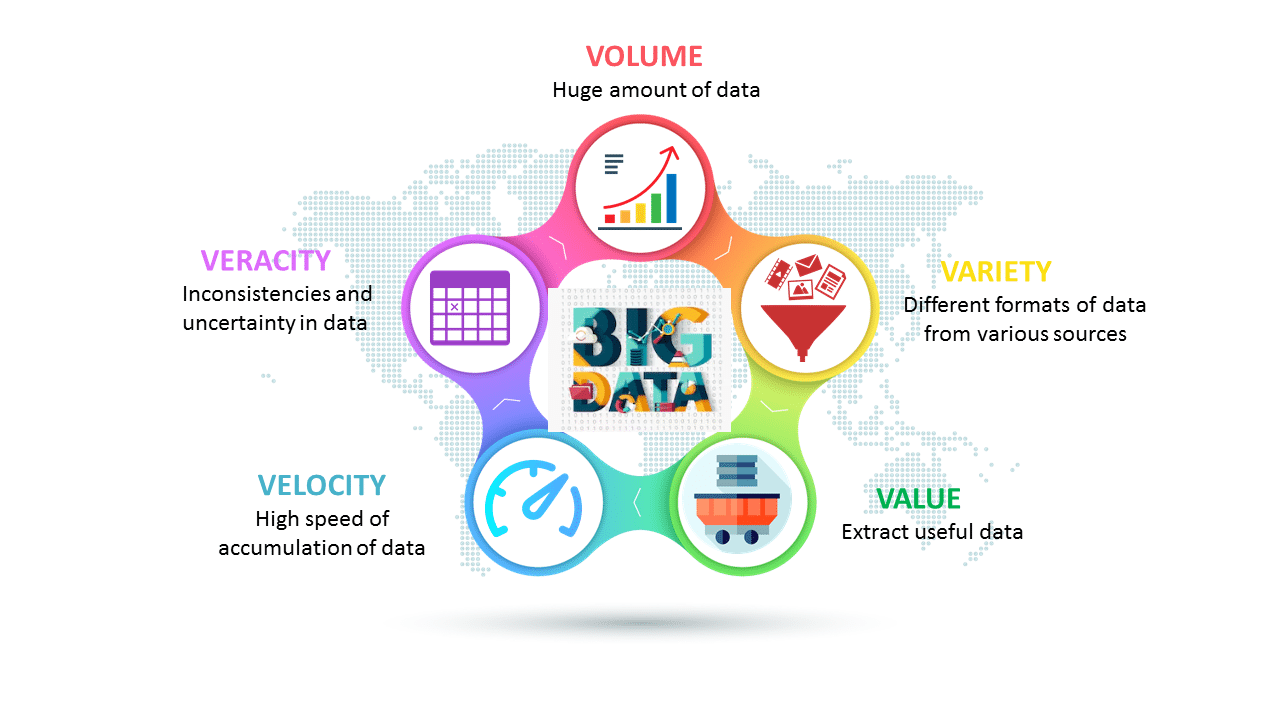
\includegraphics[width=1\textwidth]{figures/Vs}
\end{frame}

\begin{frame}{Big Data}
    y... eso tiene potencial?
    \centering
    \href{https://www.mckinsey.com/business-functions/mckinsey-digital/our-insights/big-data-the-next-frontier-for-innovation}{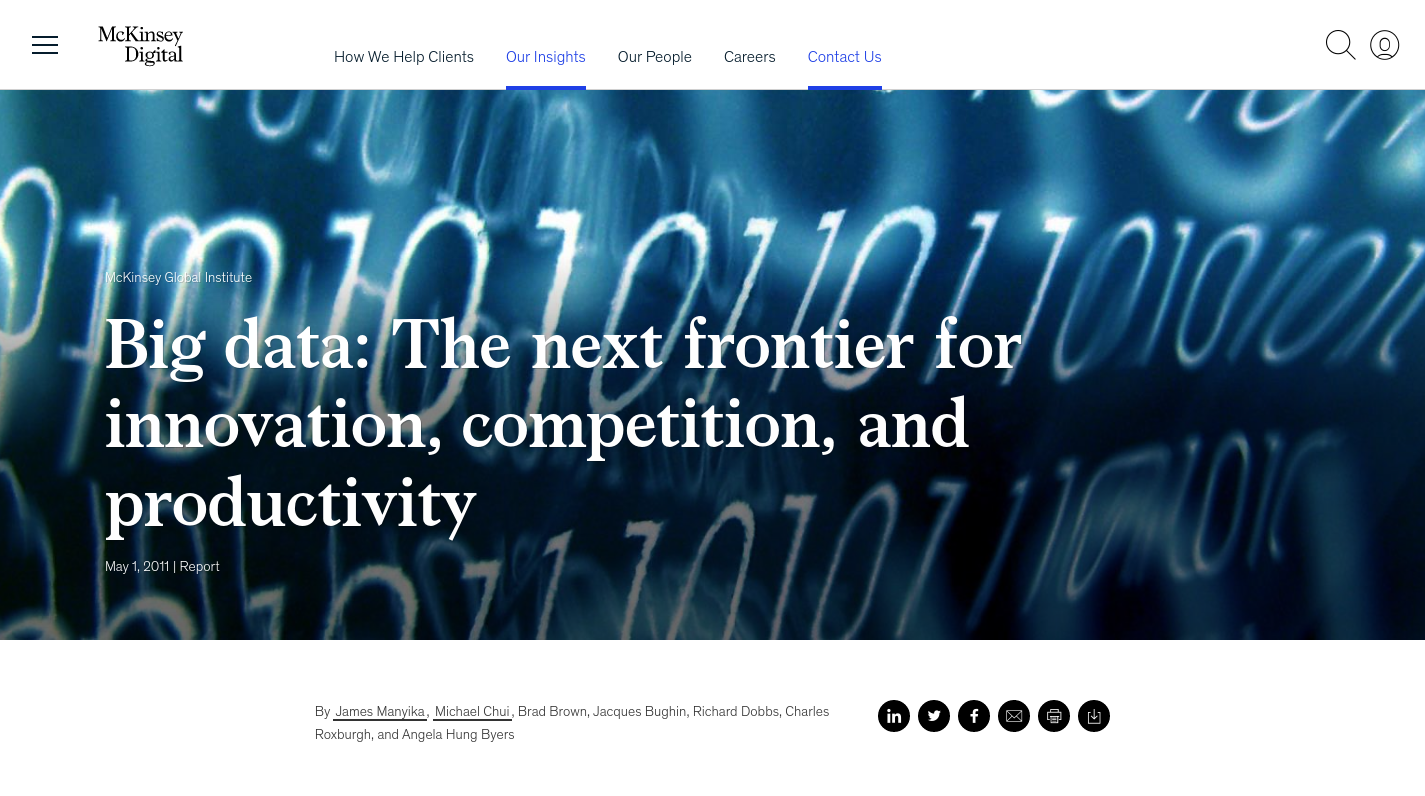
\includegraphics[width=1\textwidth]{figures/mckinsey}}
\end{frame}

\begin{frame}{Big Data}
    \begin{enumerate}
        \item En el 2009, empresas con más de 1000 empleados manejaron en promedio 200 terabytes de datos almacenados.
        \item El uso de Big Data es un componente diferenciador y crítico a la hora de la competitividad de las empresas.
        \item Hay una escasez de talento humano.  En US se necesitan entre 140K y 190K profesionales capacitados.
        \item El mercado es de USD 1 trillion para el 2020.  Solo el sector de los servicios basados en localización vale USD 600 million.
    \end{enumerate}
\end{frame}

\begin{frame}{Big Data}
    La ley de Moore? Not AnyMoore...
  \centering
  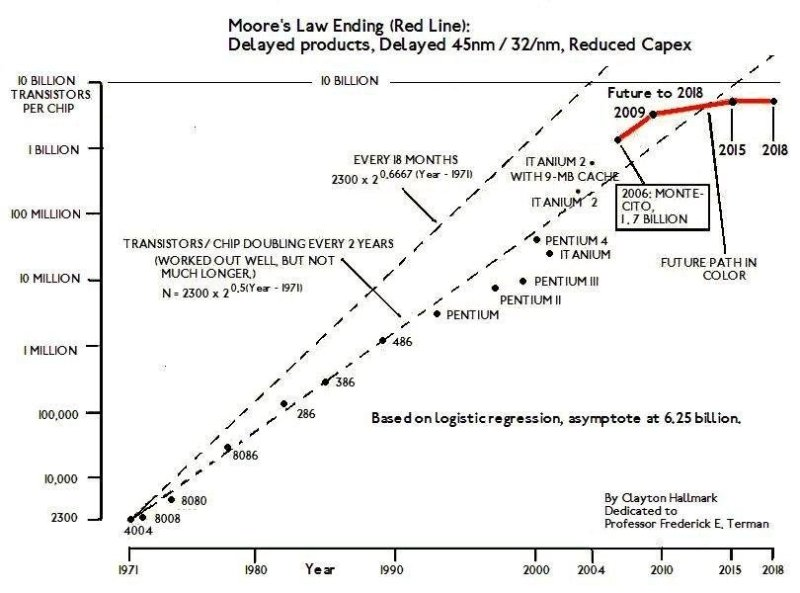
\includegraphics[width=0.8\textwidth]{figures/moore}
\end{frame}

\begin{frame}{Big Data}
    Soluciones?
    \begin{itemize}
        \item Quantum computing... \\
        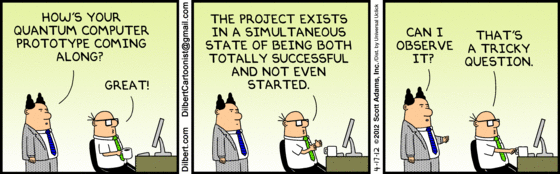
\includegraphics[width=0.7\textwidth]{figures/quantum} 
    \end{itemize}
    {\tiny 
        \begin{itemize}
         \item Cómo va tu proyecto de computador cuántico?
         \item Genial!
         \item El proyecto existe en un estado simultaneo donde, al mismo tiempo, es un éxito total y otro donde ni siquiera he empezado.
         \item Puedo ver?
         \item Esa es la pregunta!
        \end{itemize}
    }
\end{frame}

\begin{frame}{Big Data}
    Soluciones?
    \begin{itemize}
        \item Sistemas distribuidos... \\
        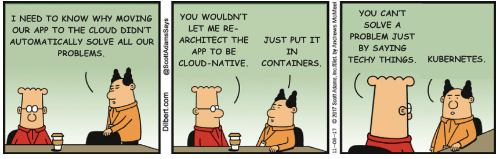
\includegraphics[width=0.7\textwidth]{figures/distributed} 
    \end{itemize}
    {\tiny 
        \begin{itemize}
         \item Necesito saber porqué migrar nuestra aplicación a la nube no resuelve automáticamente todos nuestros problemas.
         \item Tu no me dejaste re-estructurar la app para que sea nativa en la nube.
         \item Solo colocala en un container.
         \item Tu no puedes resolver los problemas solo usando términos técnicos.
         \item Kubernetes!
        \end{itemize}
    }    
\end{frame}

\begin{frame}{Big Data}
The billion dollar data centers y el famoso `MapReduce'...
  \centering
  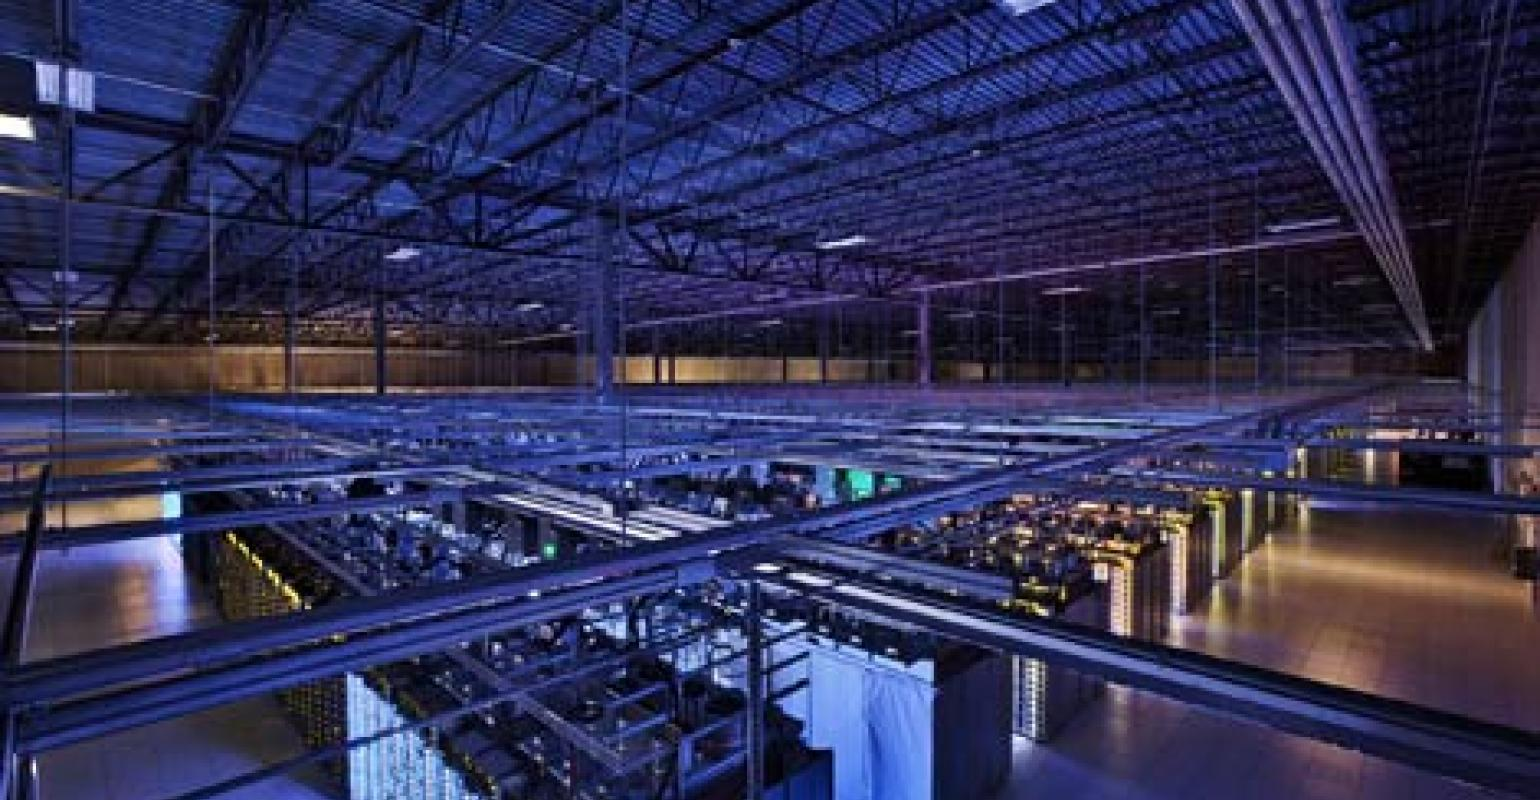
\includegraphics[width=\textwidth]{figures/datacenter}
\end{frame}

\begin{frame}{Big Data}
The billion dollar data centers y el famoso `MapReduce'...
  \centering
  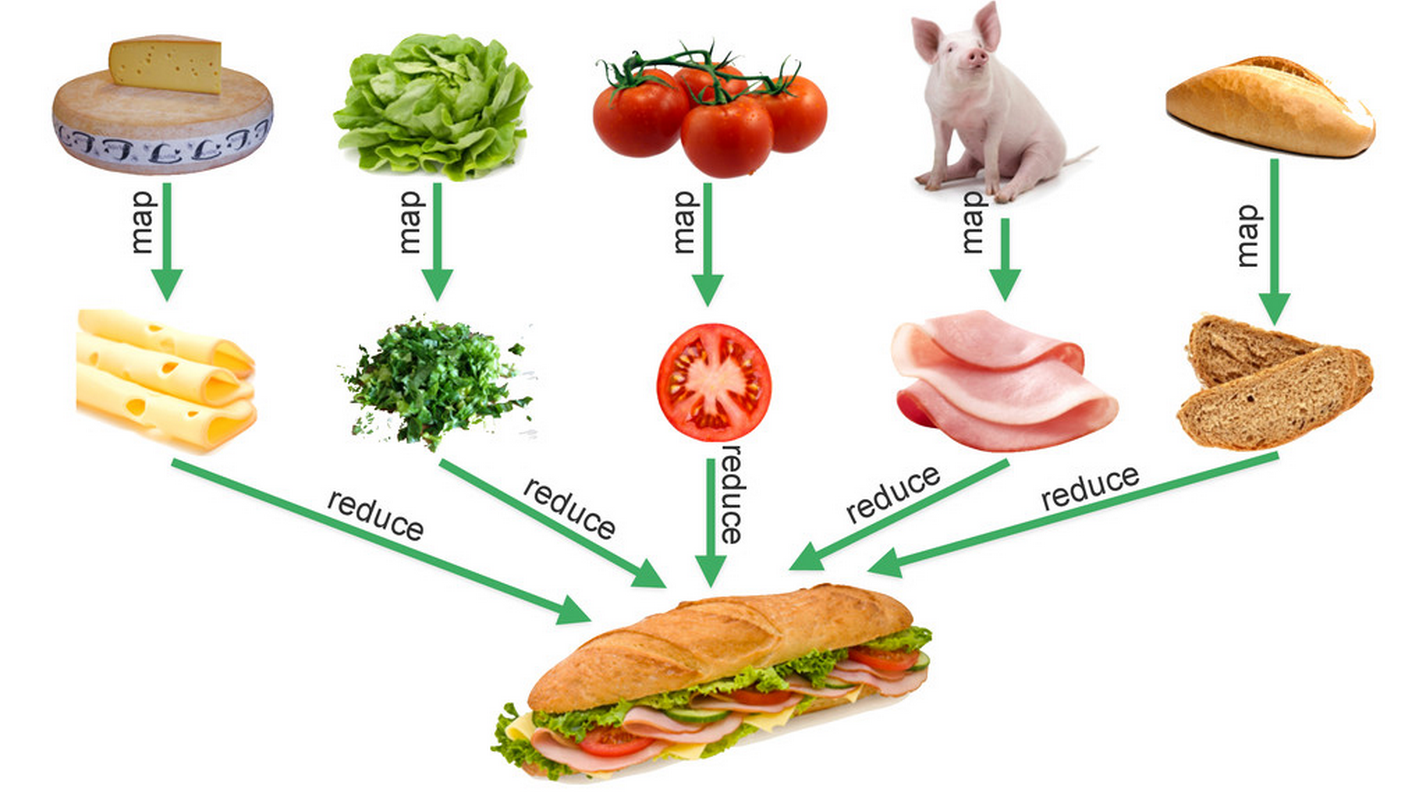
\includegraphics[width=\textwidth]{figures/mapreduce}
\end{frame}

\section{Big Spatial Data}

\begin{frame}{Big Spatial Data}
    Spatial is Special... \\
    \centering
    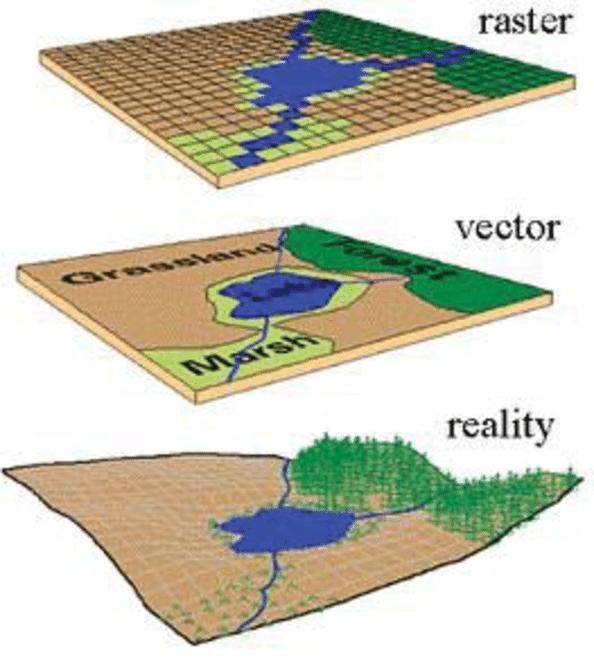
\includegraphics[width=0.5\textwidth]{figures/geomodels}
\end{frame}

\begin{frame}{Big Spatial Data}
    Maps are Special... \\
    \begin{enumerate}
        \item Los mapas ofrecen datos ricos en información.
        \item Espacialización de la información (location - location - location).
        \item Geomarketing (Minority Report).
        \item Interfaces Humano - Robot (UAVs).
        \item Son plataformas de integración (IoT).
    \end{enumerate}
\end{frame}

\begin{frame}{Big Spatial Data}
    Geodata are Special... \\
    \begin{enumerate}
        \item Nuevos tipos de datos (Point - Line - Polygon).
        \item Nuevas operaciones (Intersection - Covered by - Touch).
        \item Nuevas particularidades (Spatial indexing - Spatial joins).
        \item Nuevos conceptos (Topology - CRS).
    \end{enumerate}
\end{frame}

\begin{frame}{Big Spatial Data}
  \centering
  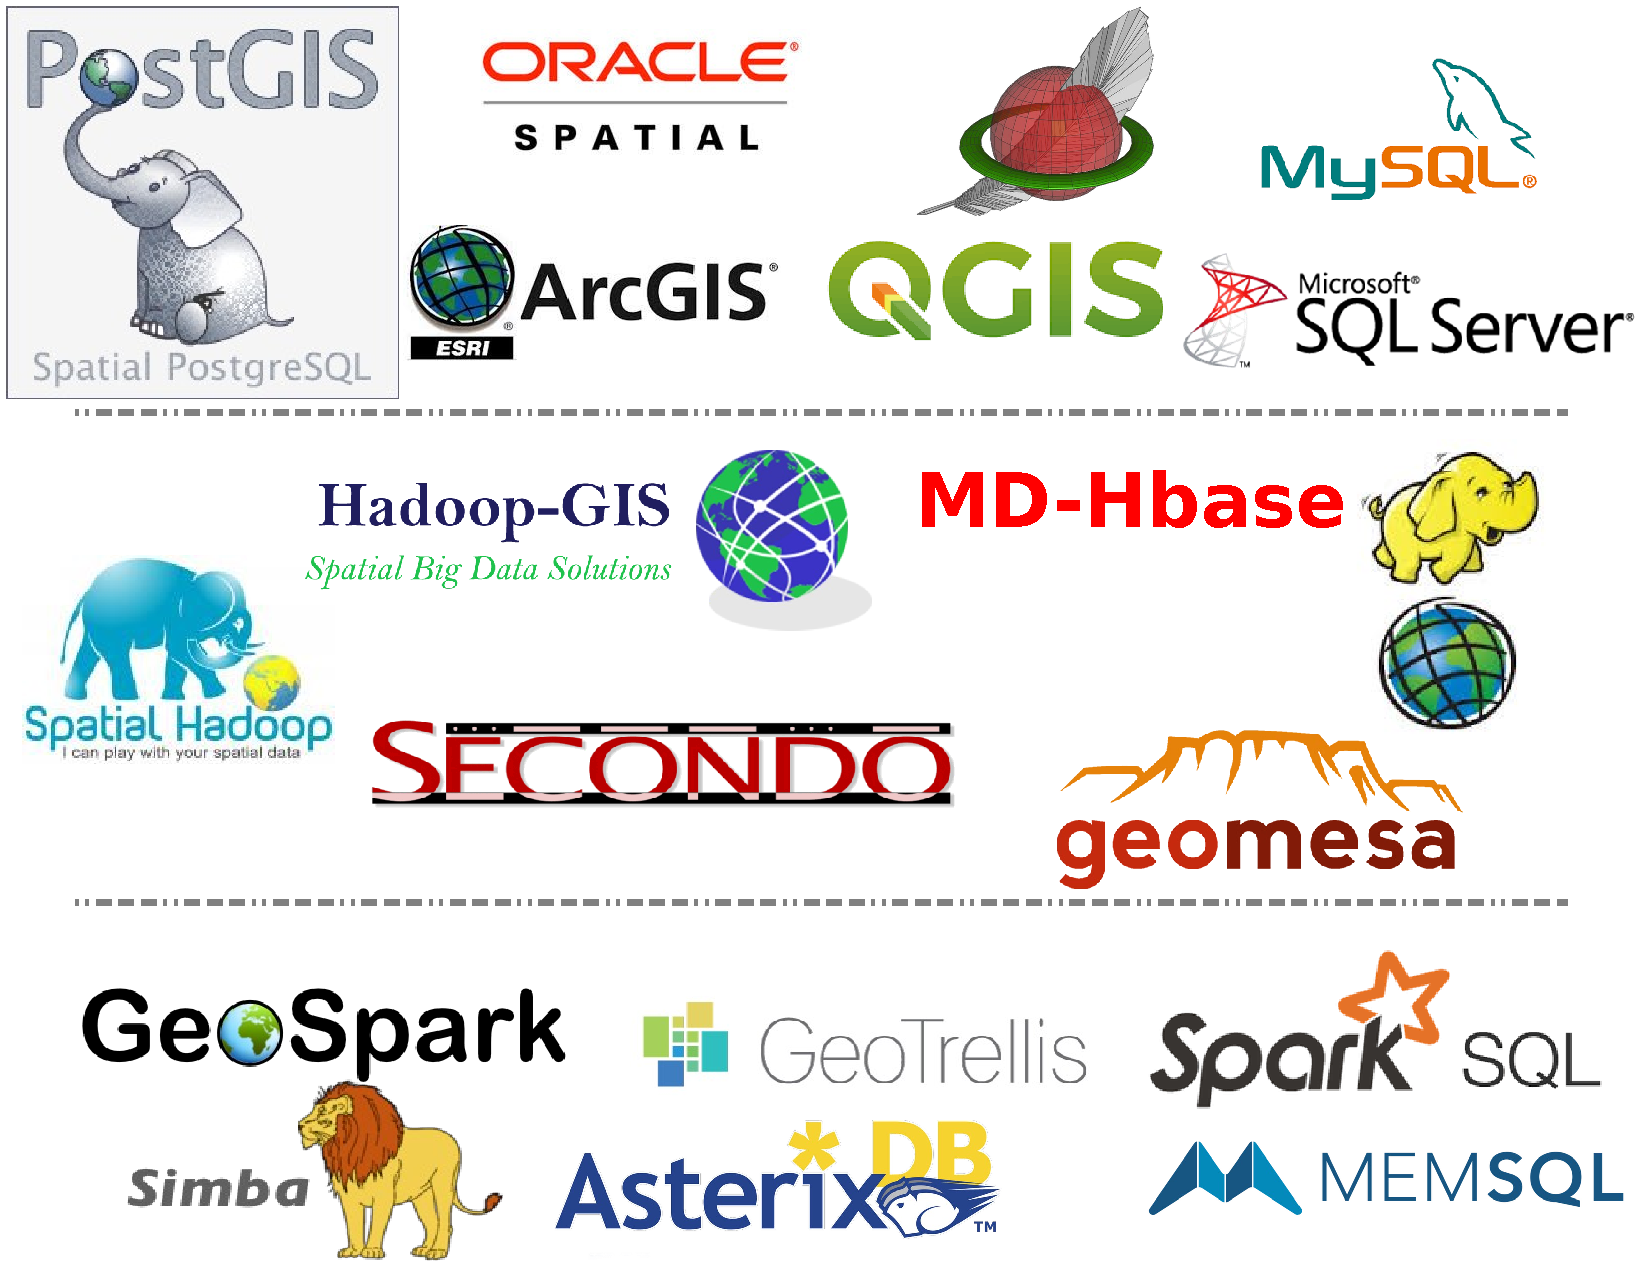
\includegraphics[clip, trim=0cm 14cm 0cm 0cm, width=0.85\linewidth]{figures/logos}
\end{frame}

\begin{frame}[noframenumbering]{Big Spatial Data}
  \centering
  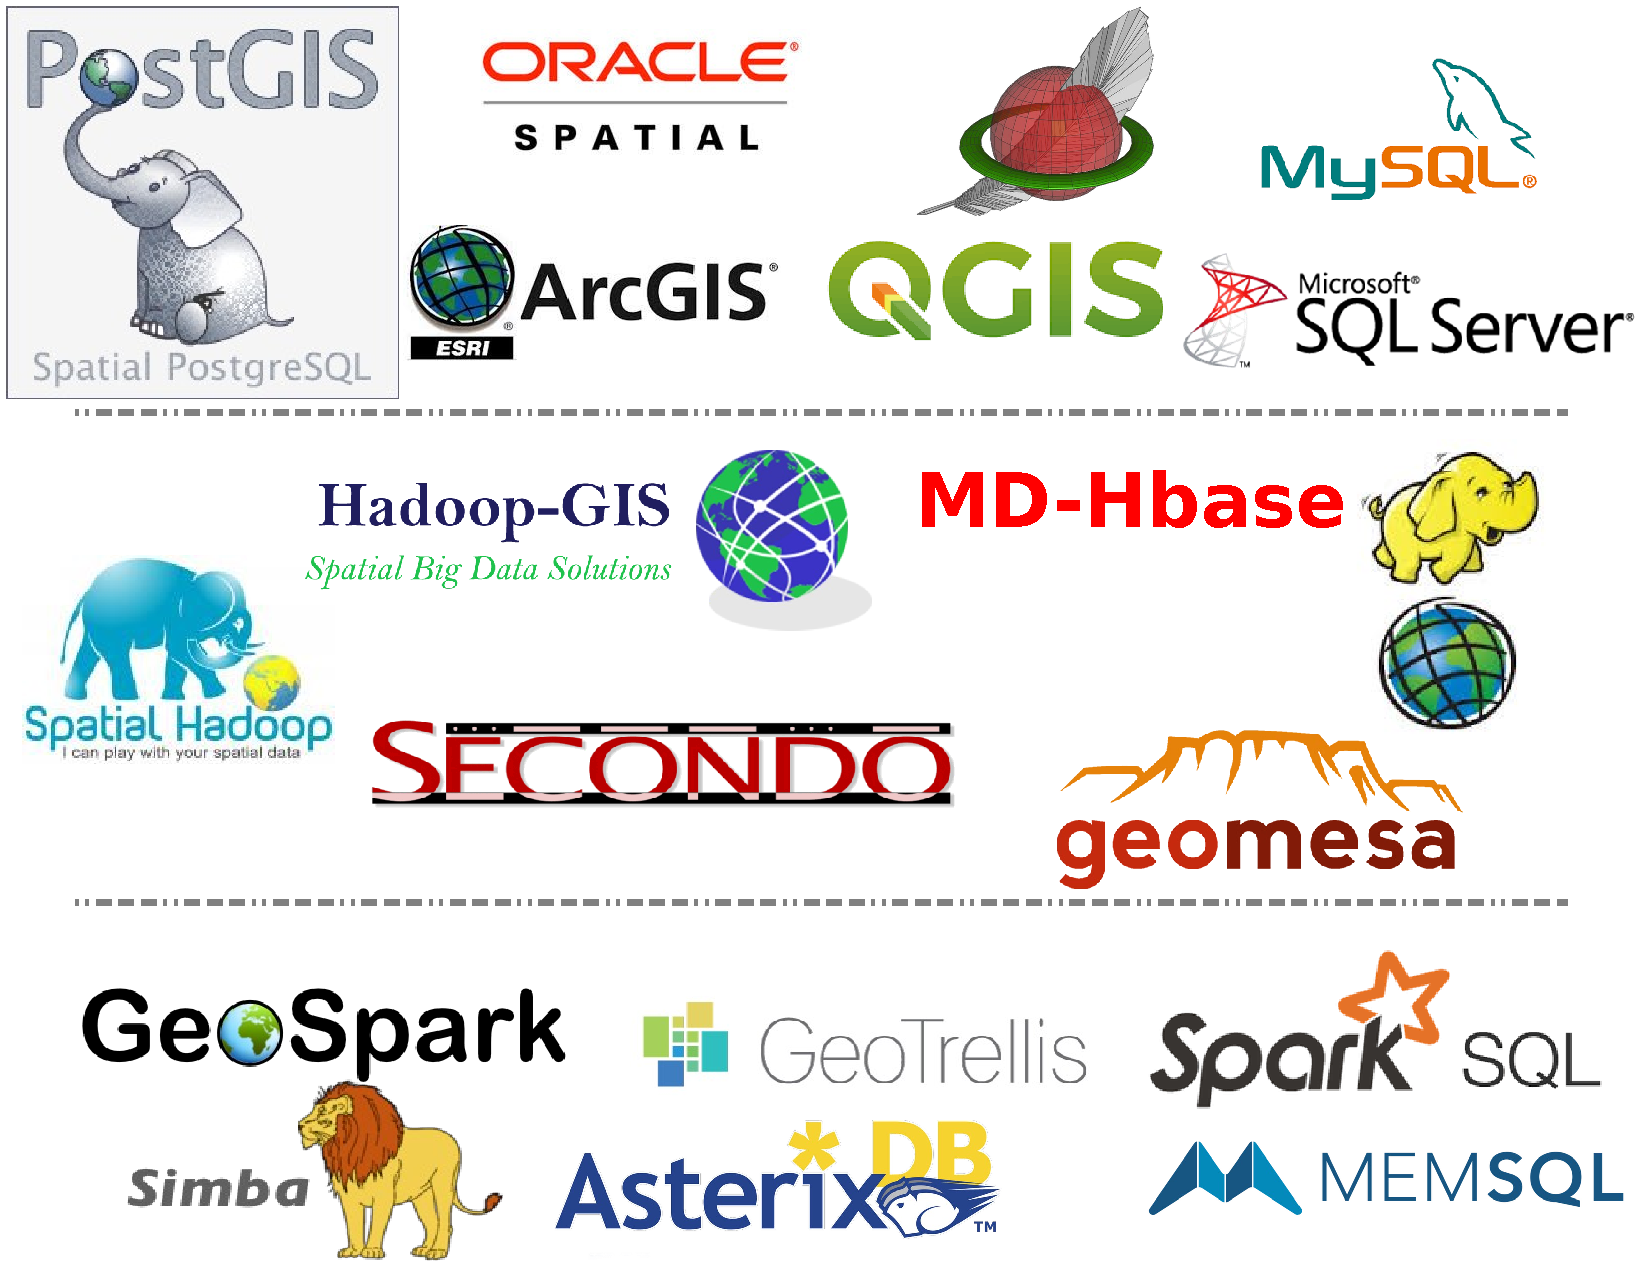
\includegraphics[clip, trim=0cm 6cm 0cm 0cm, width=0.85\linewidth]{figures/logos}
\end{frame}

\begin{frame}[noframenumbering]{Big Spatial Data}
  \centering
  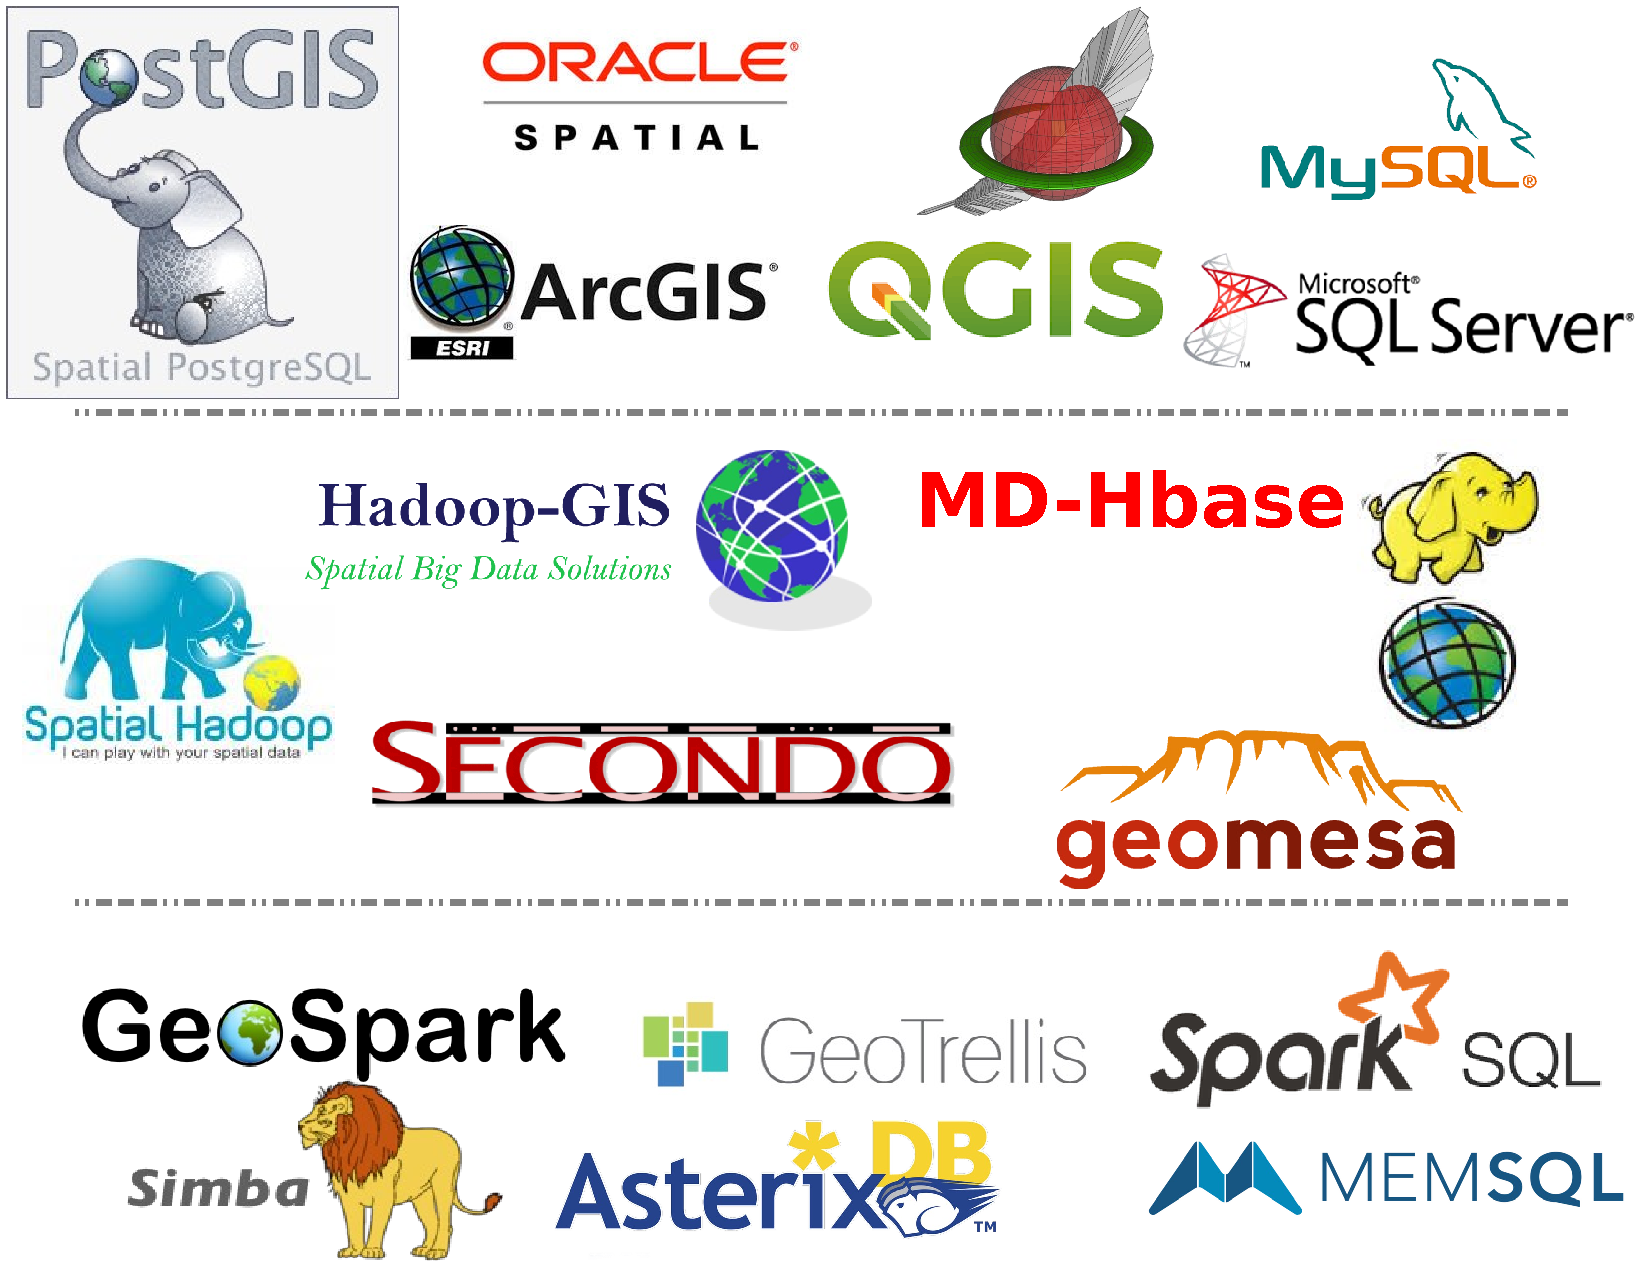
\includegraphics[clip, trim=0cm 0cm 0cm 0cm, width=0.85\linewidth]{figures/logos}
\end{frame}

\begin{frame}{Big Spatial Data}
    \begin{itemize}
        \item Geomesa \url{https://www.geomesa.org/}
        \item AsterixDB \url{https://asterixdb.apache.org/}
        \item GeoSpark \url{https://datasystemslab.github.io/GeoSpark/}
    \end{itemize}
\end{frame}

\section{La Era del Big Spatial Data}

\begin{frame}{La Era del Big Spatial Data}
    \centering
    \includemedia[
        width=0.5\linewidth,
        height=0.5\linewidth,
        activate=pageopen,
        addresource=figures/landsat.mp4,
        flashvars={source=figures/landsat.mp4}
    ]{}{VPlayer.swf}\\
    
    Landsat entrega más de 1200 imagenes y un total de 1TB diario.
\end{frame}

\begin{frame}{La Era del Big Spatial Data}
  \centering
  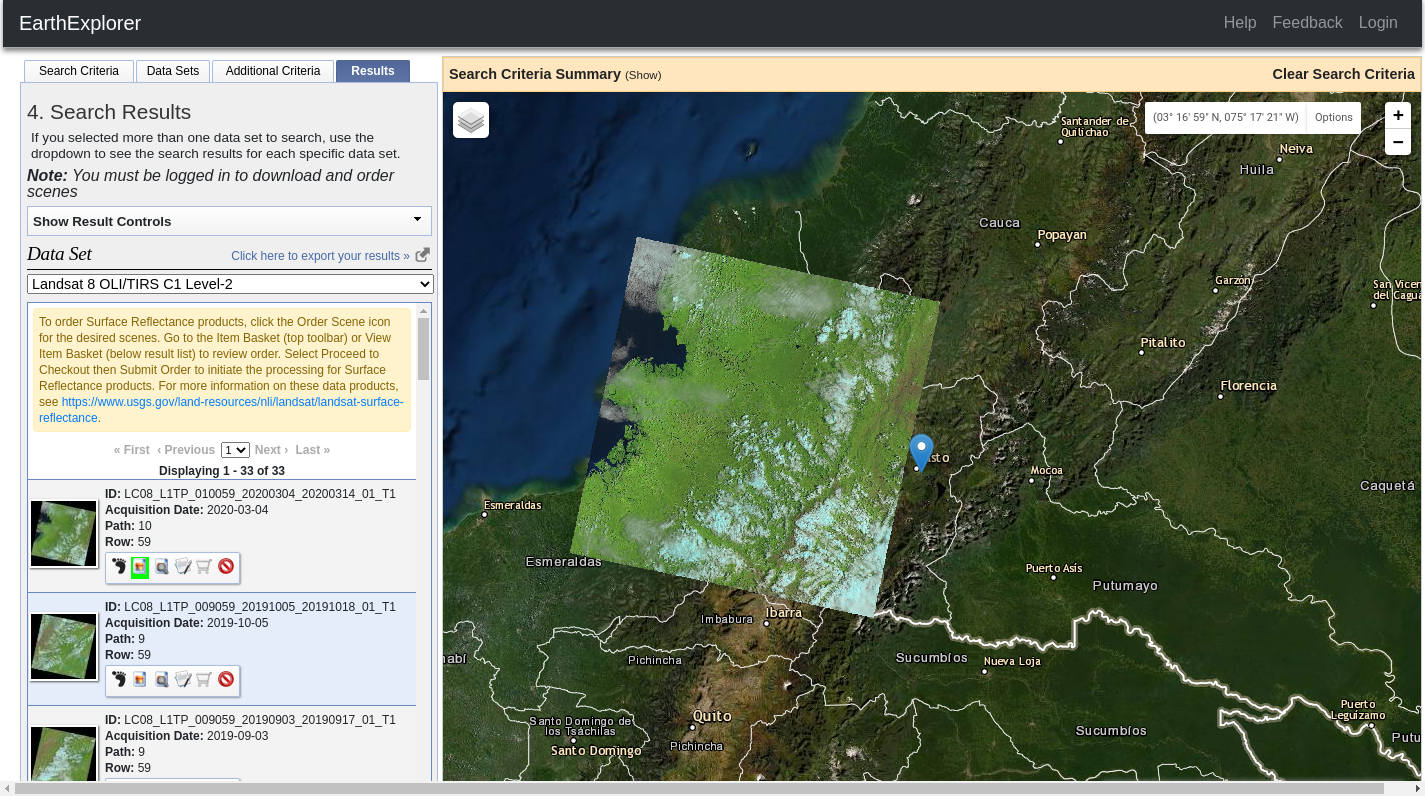
\includegraphics[width=\textwidth]{figures/ee}
  \blfootnote{\url{https://earthexplorer.usgs.gov/}}
\end{frame}

\begin{frame}{La Era del Big Spatial Data}
  \centering
  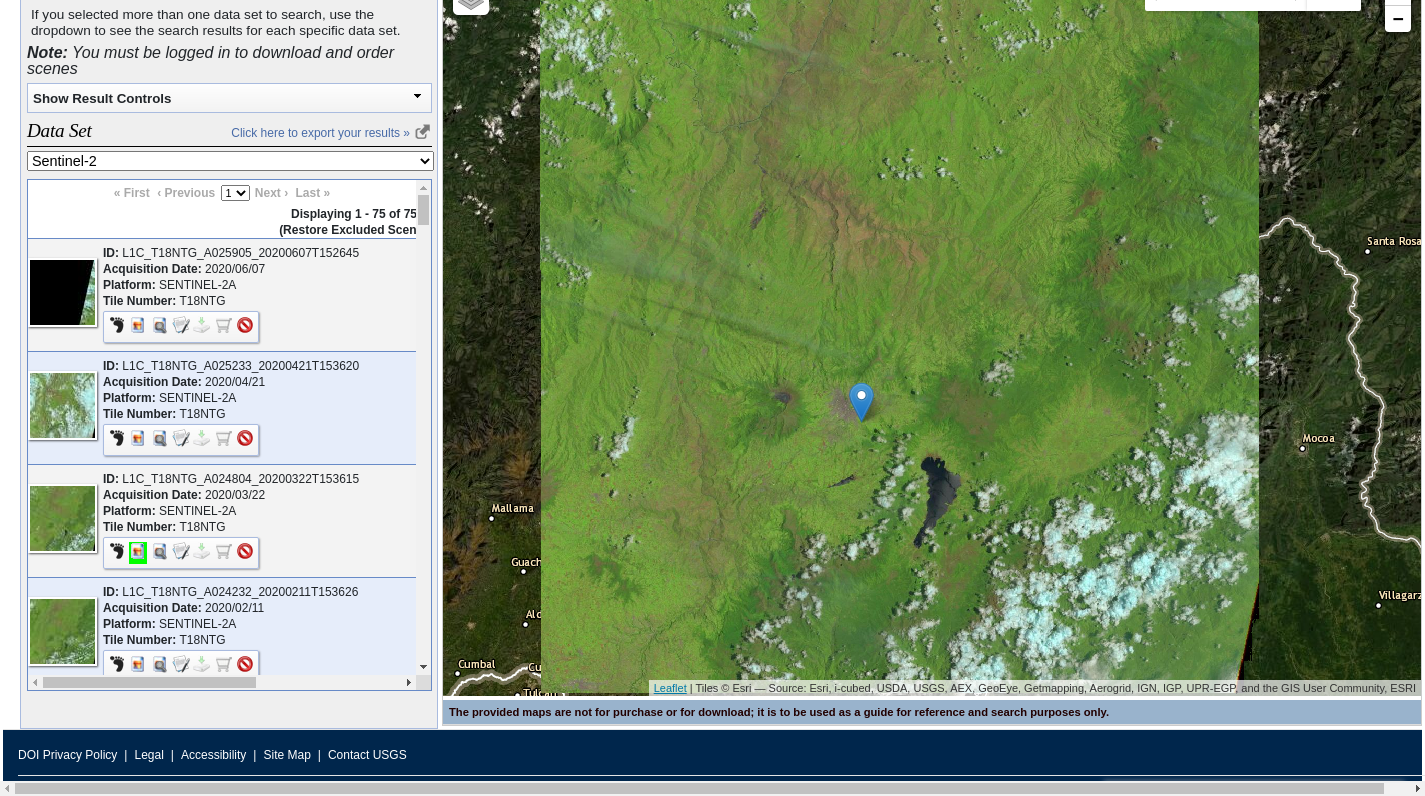
\includegraphics[width=\textwidth]{figures/sentinel}
  \blfootnote{\url{https://earthexplorer.usgs.gov/}}
\end{frame}

\begin{frame}{La Era del Big Spatial Data}
    \centering
    \includemedia[
        width=0.5\linewidth,
        height=0.5\linewidth,
        activate=pageopen,
        addresource=figures/osm2.mp4,
        flashvars={source=figures/osm2.mp4}
    ]{}{VPlayer.swf}\\
    
    OSM recopila más de 1.2TB de datos vectoriales en formato abierto.
\end{frame}

\begin{frame}{La Era del Big Spatial Data}
  \centering
  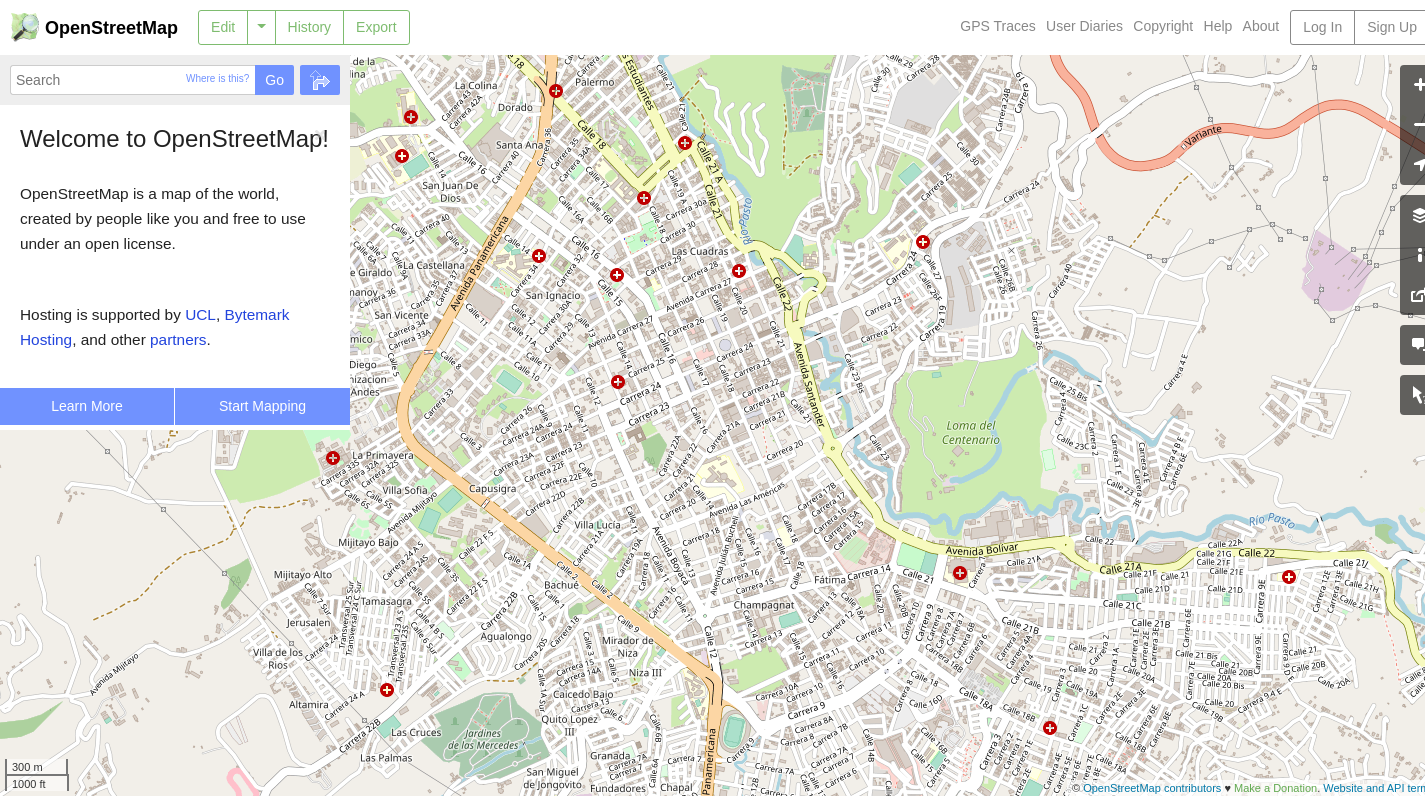
\includegraphics[width=\textwidth]{figures/osm}
  \blfootnote{\url{https://www.openstreetmap.org/}}
\end{frame}

\begin{frame}{La Era del Big Spatial Data}
  \centering
  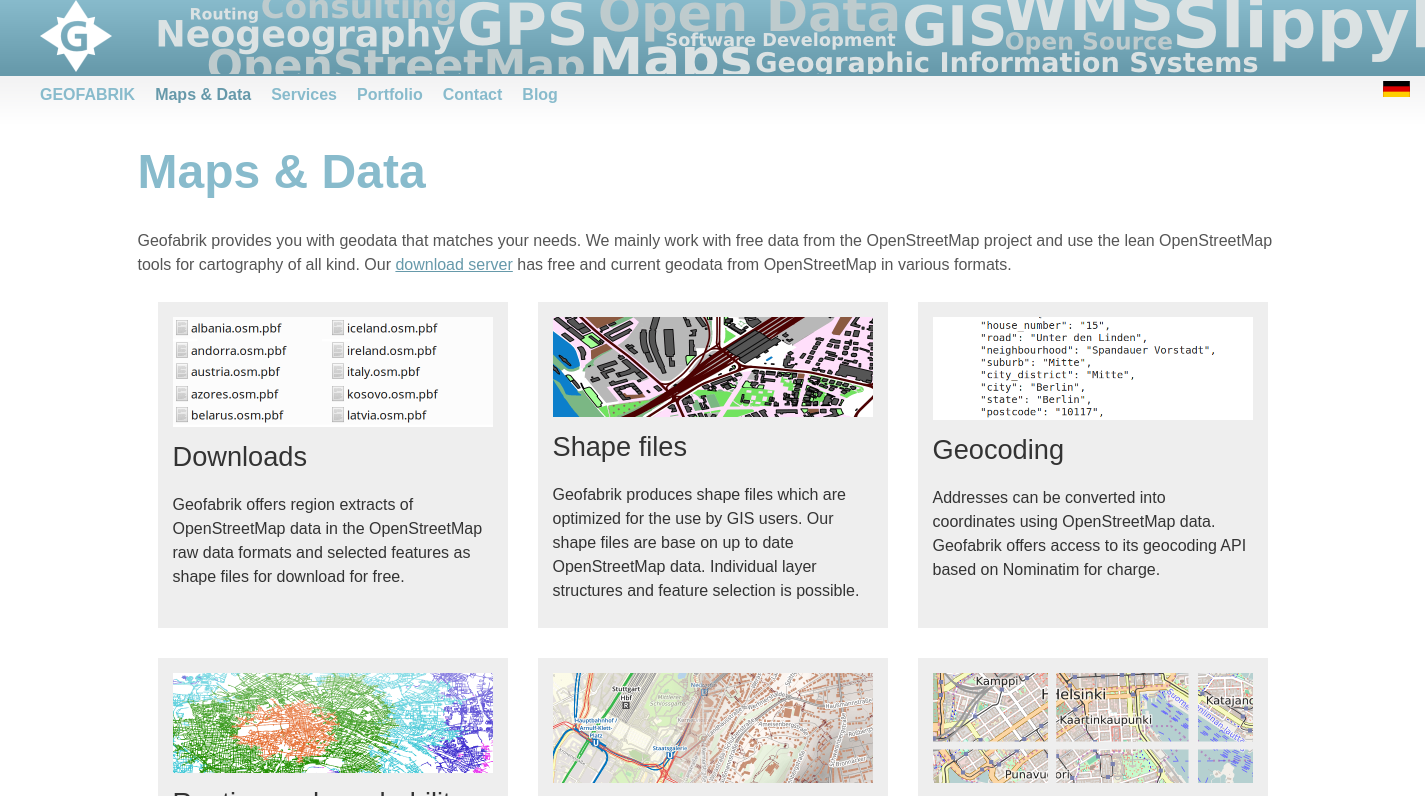
\includegraphics[width=\textwidth]{figures/geofabrik}
  \blfootnote{\url{https://www.geofabrik.de/data/index.html}}
\end{frame}

\begin{frame}{La Era del Big Spatial Data}
  \centering
  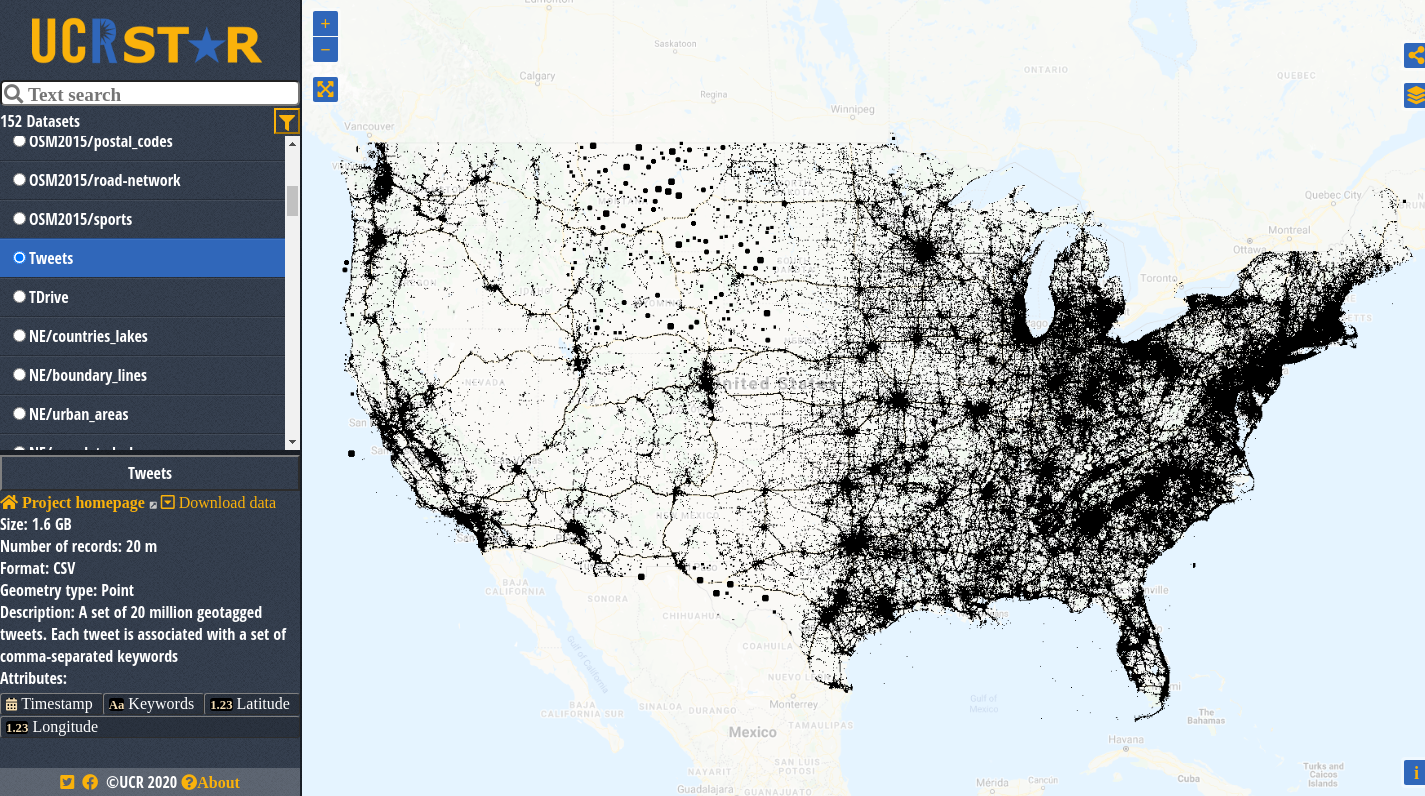
\includegraphics[width=\textwidth]{figures/star}
  \blfootnote{\url{https://star.cs.ucr.edu/}}
\end{frame}

\begin{frame}{La Era del Big Spatial Data}
  \centering
  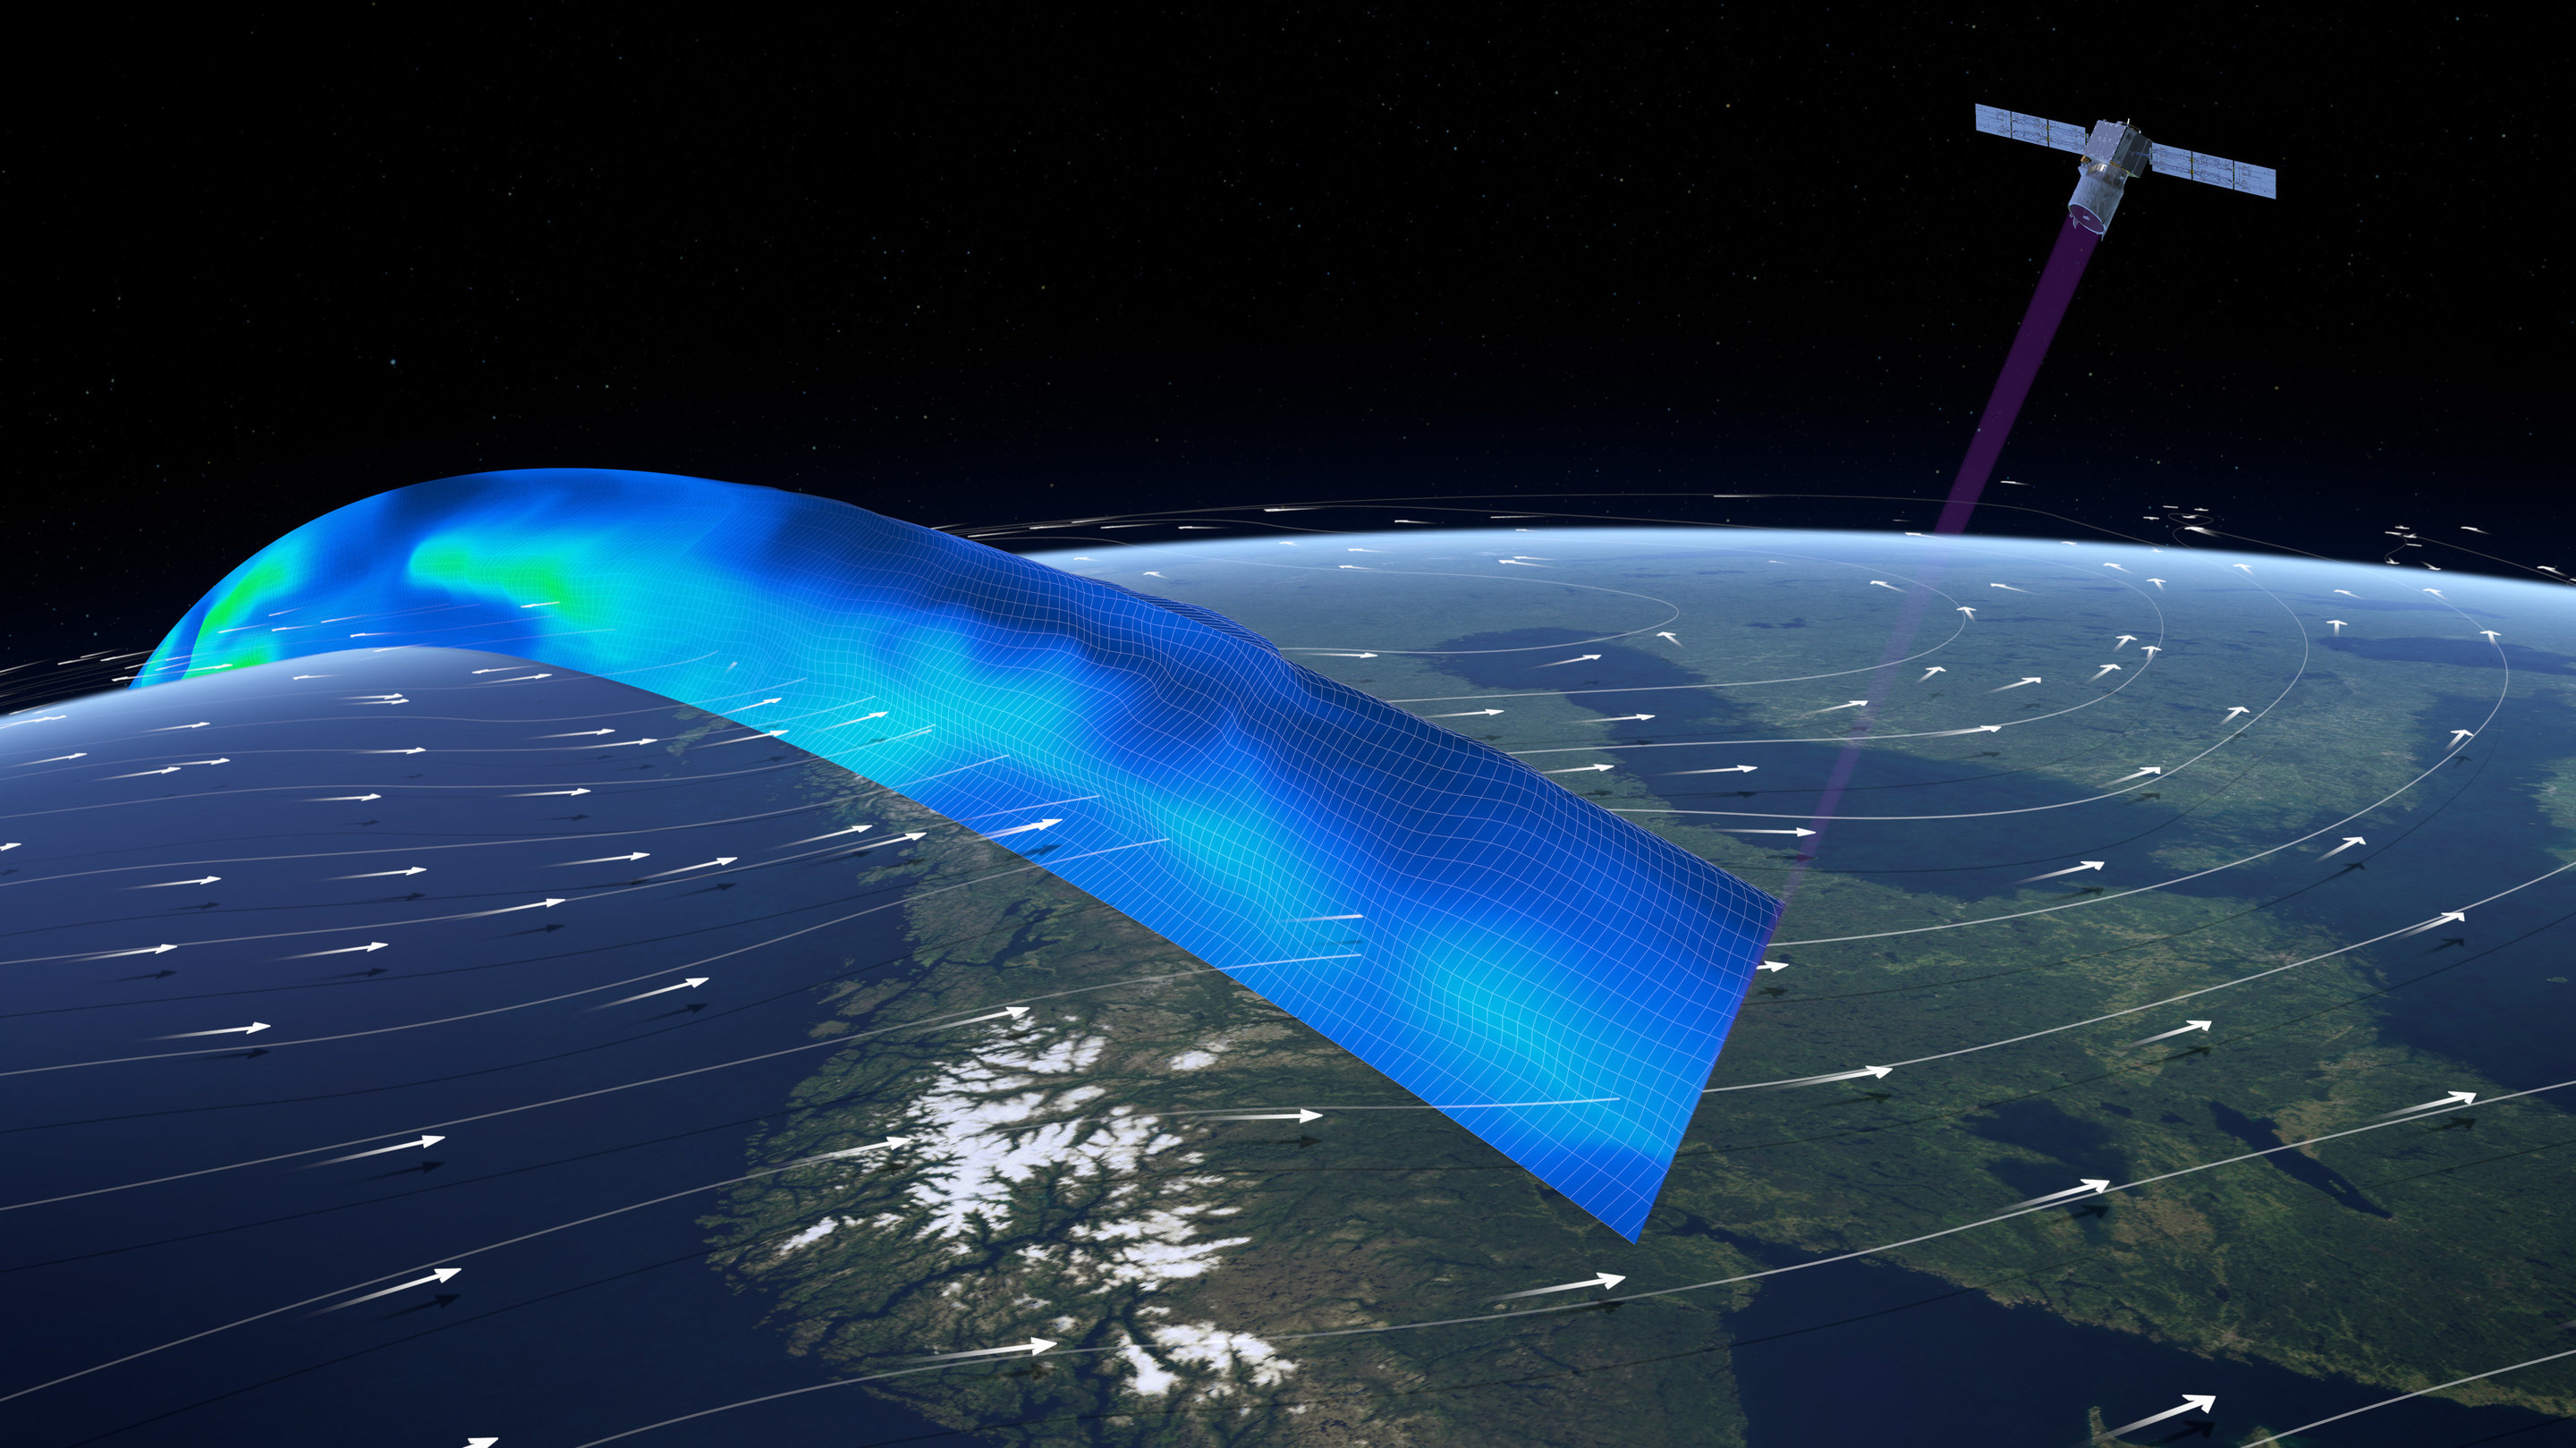
\includegraphics[width=\textwidth]{figures/aeolus}
  \blfootnote{\url{https://www.esa.int/Applications/Observing_the_Earth/Aeolus}}
\end{frame}

\begin{frame}{La Era del Big Spatial Data}
  \centering
  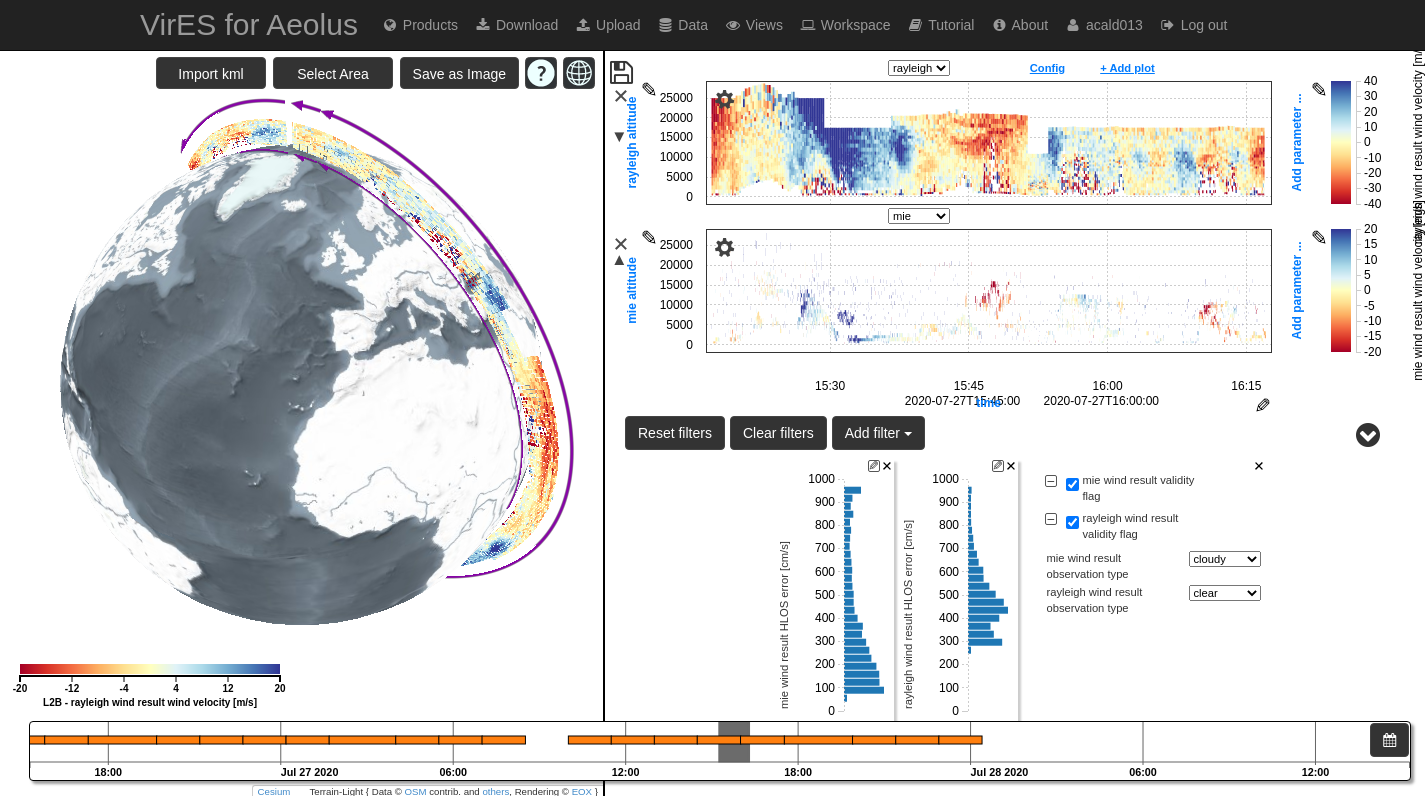
\includegraphics[width=\textwidth]{figures/vires}
  \blfootnote{\url{https://aeolus.services/}}
\end{frame}

\begin{frame}{La Era del Big Spatial Data}
  \centering
  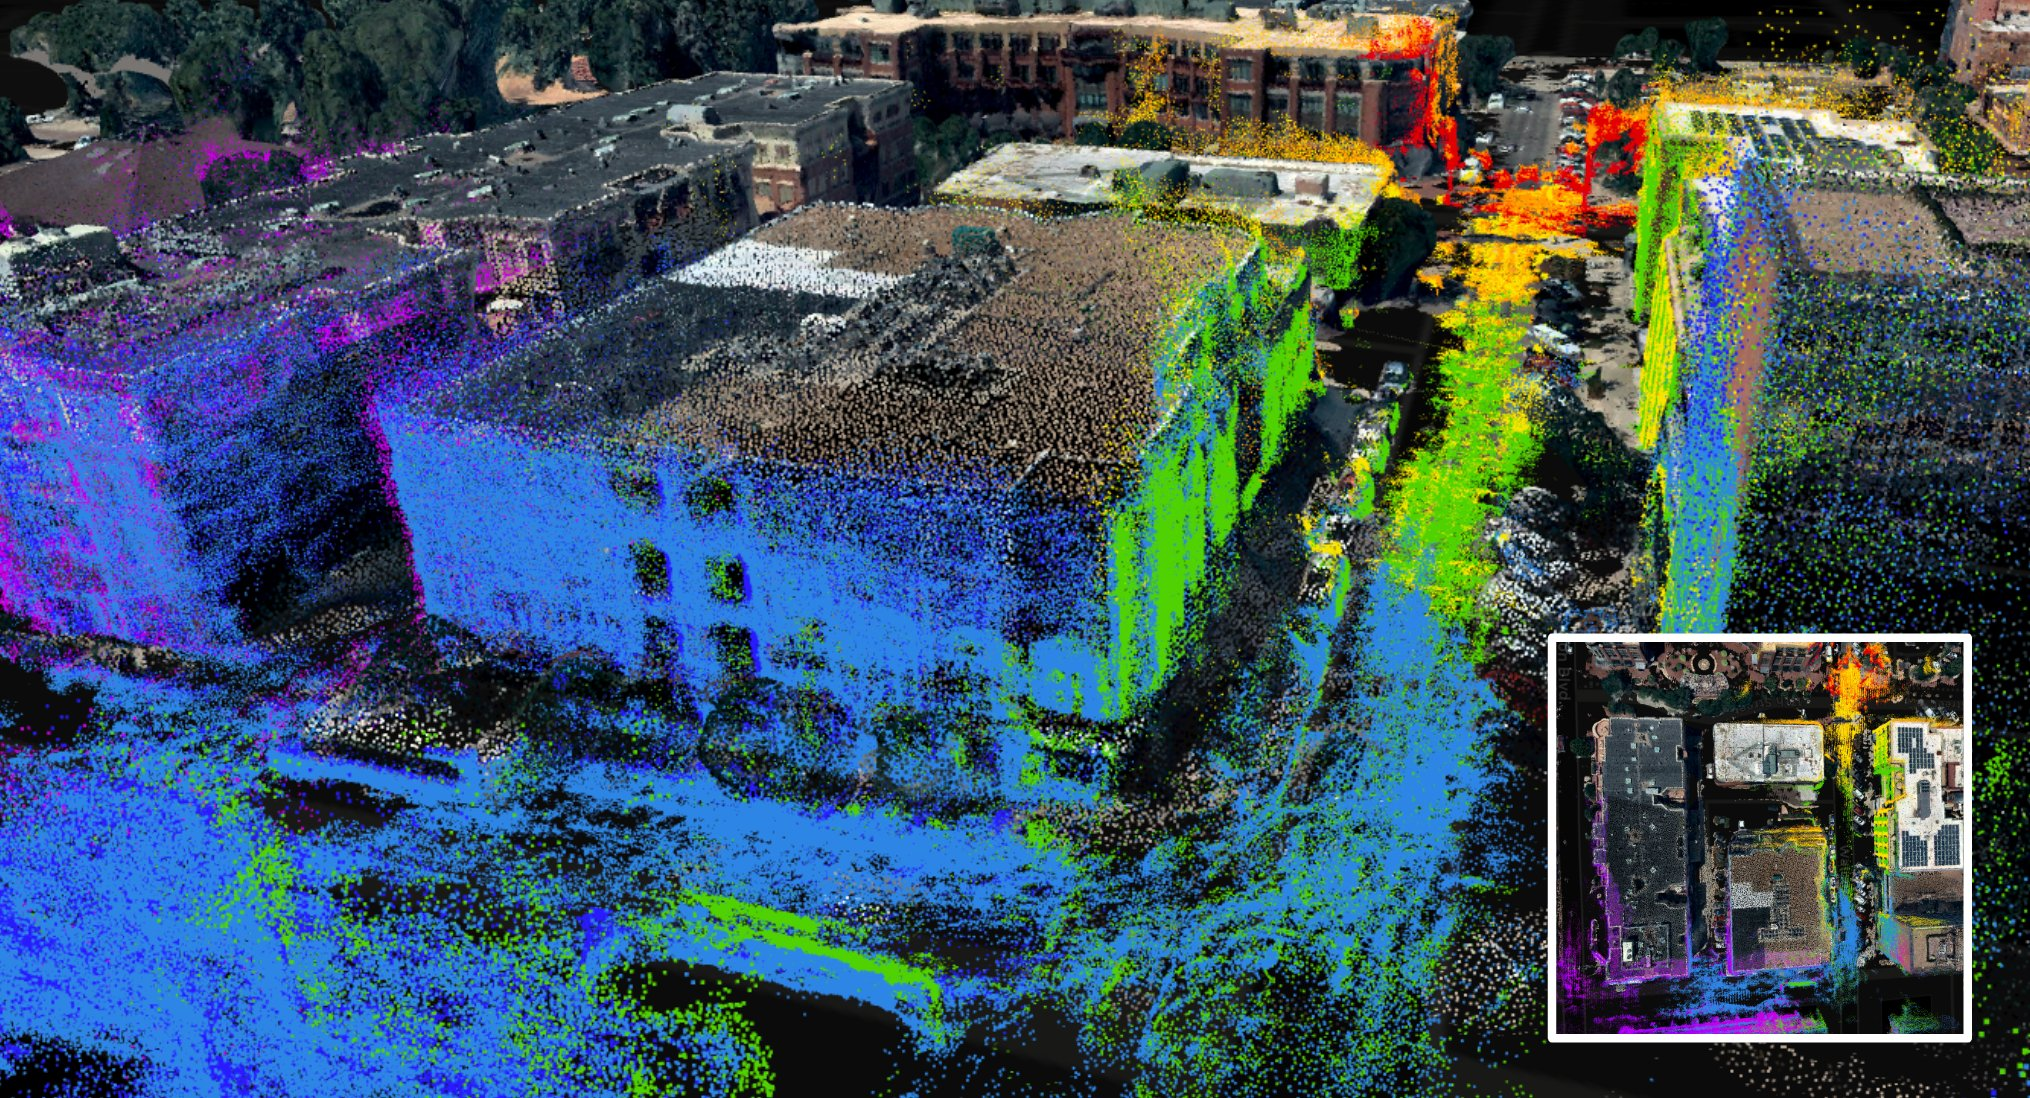
\includegraphics[width=\textwidth]{figures/lidar}
\end{frame}

\begin{frame}{La Era del Big Spatial Data}
  \centering
  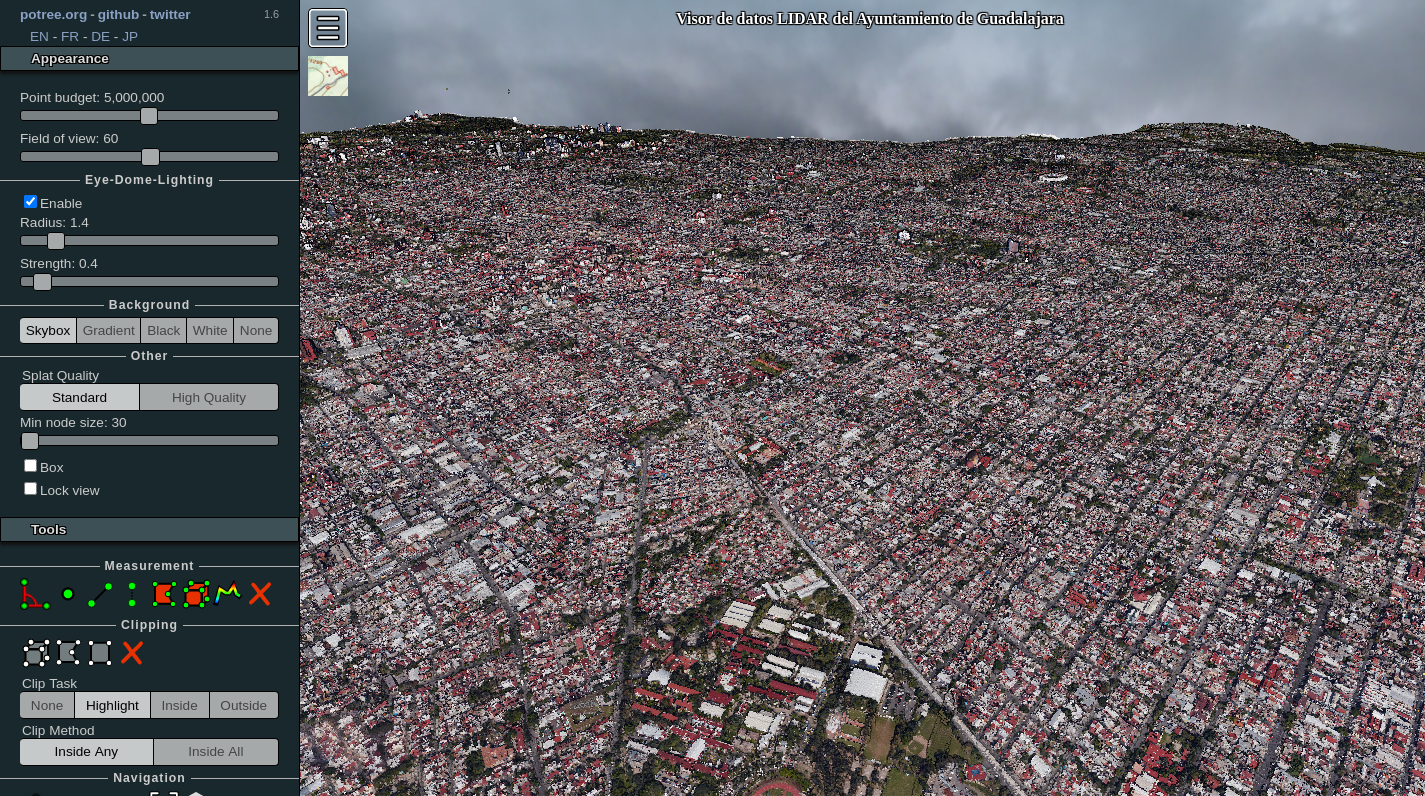
\includegraphics[width=\textwidth]{figures/guadalajara}
  \blfootnote{\url{http://lidar.guadalajara.gob.mx/}}
\end{frame}

\begin{frame}{La Era del Big Spatial Data}
  \centering
  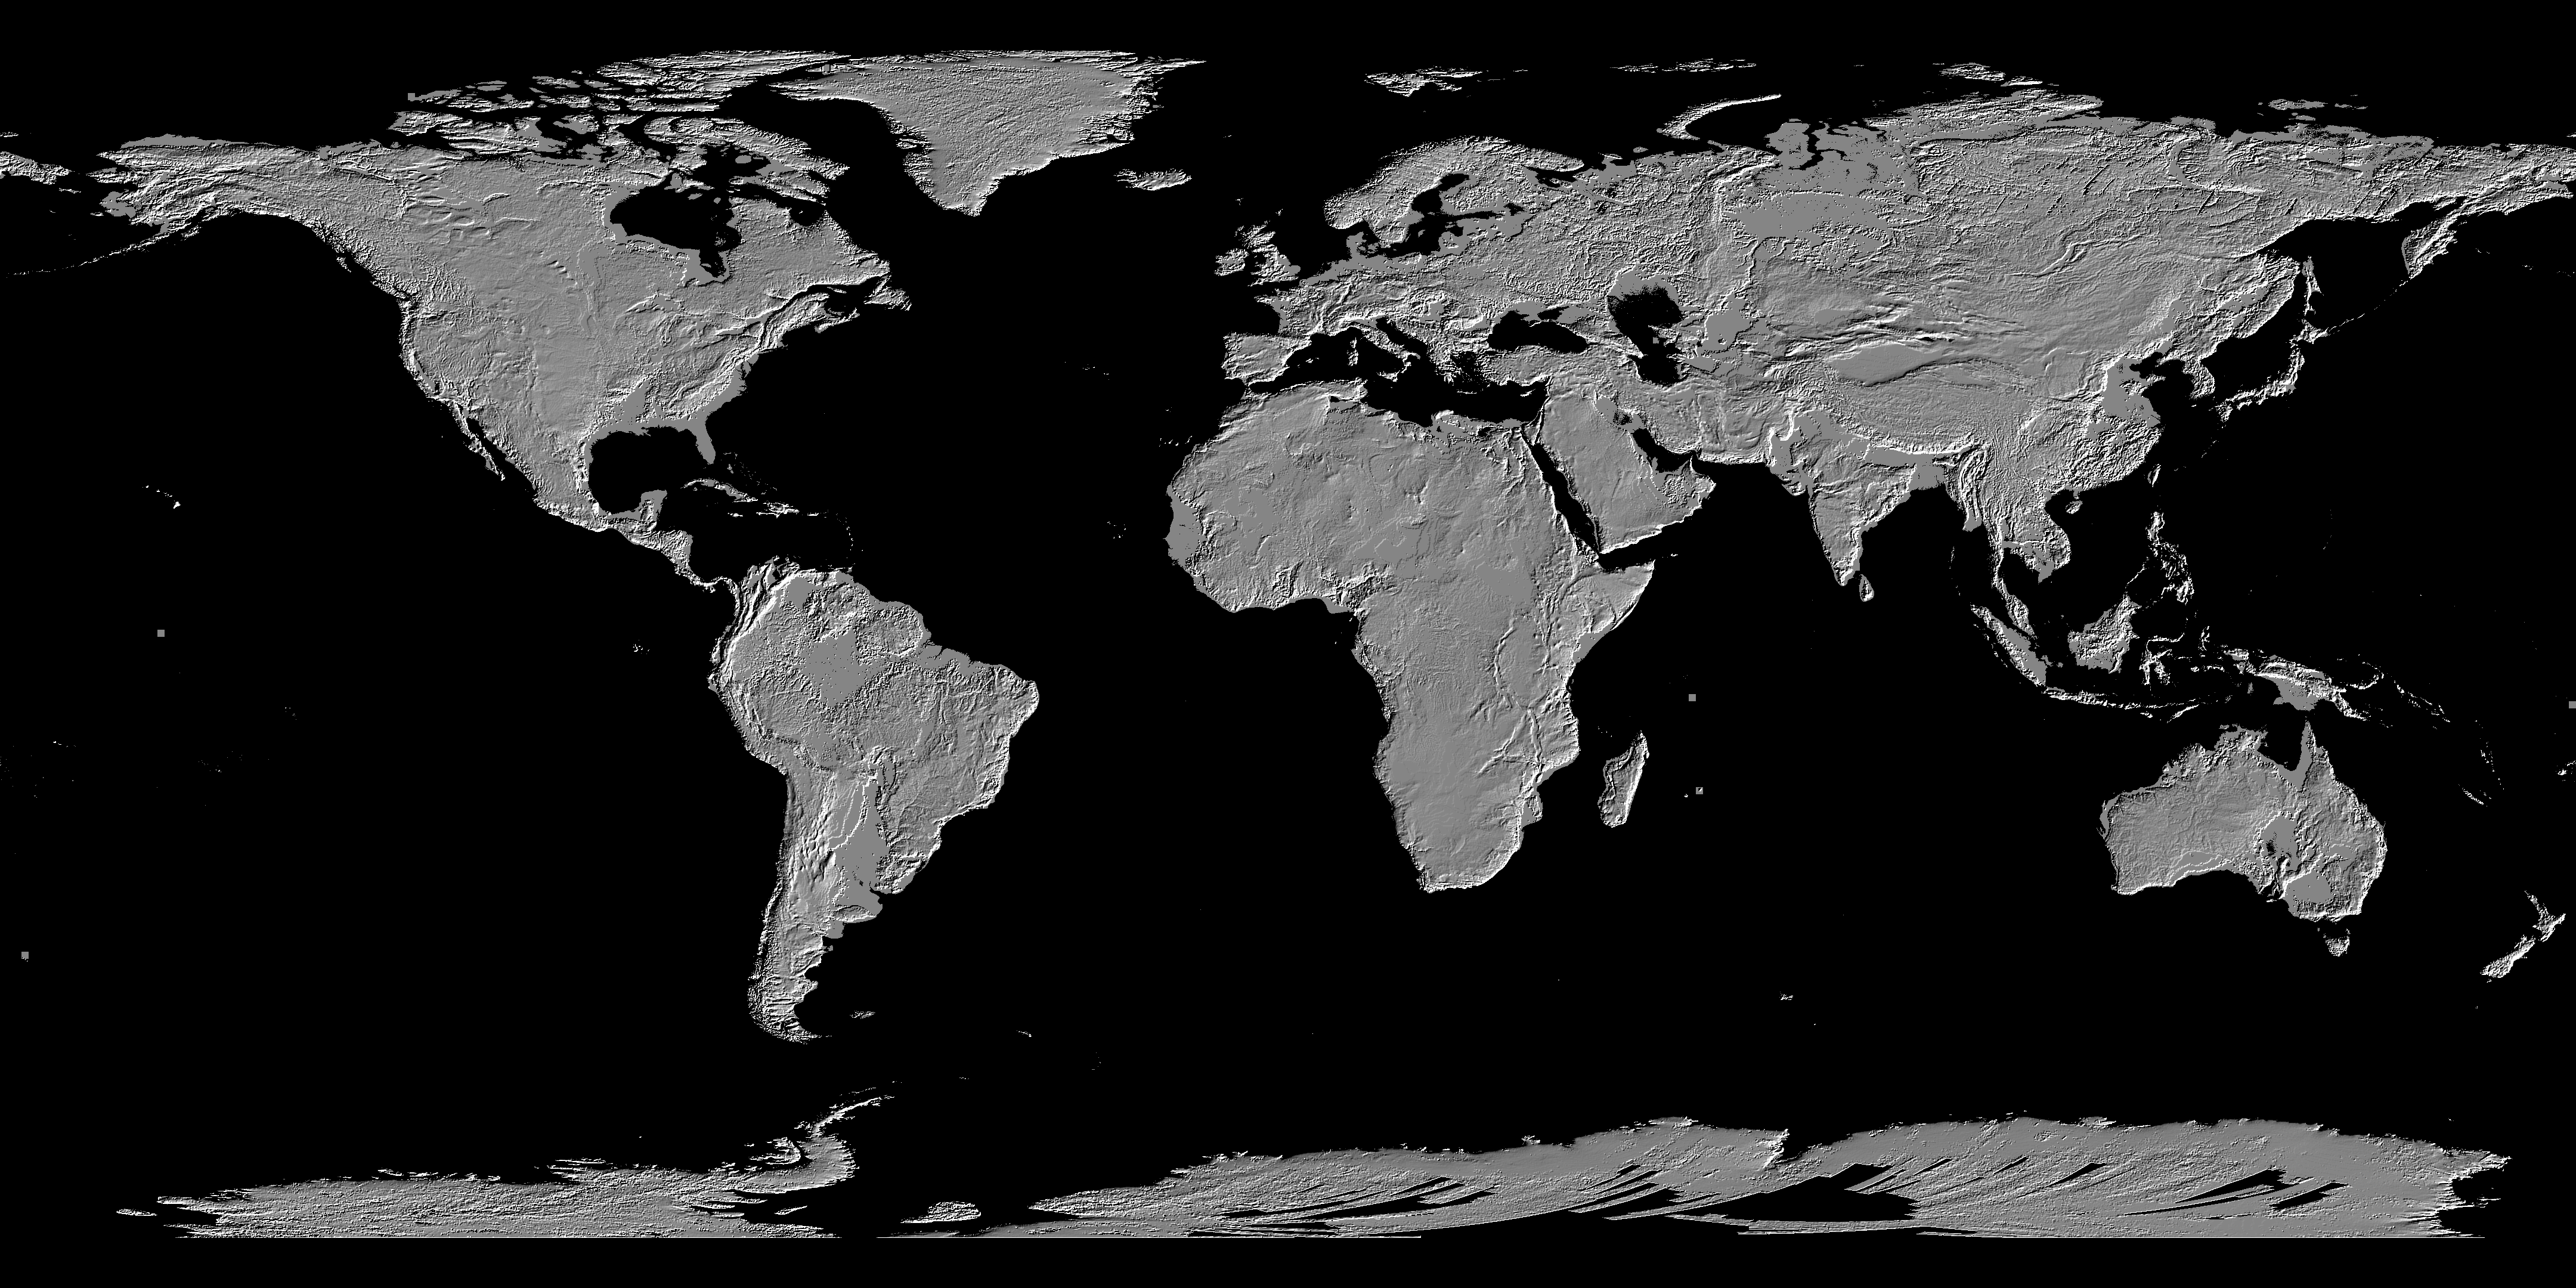
\includegraphics[width=\textwidth]{figures/asterdem}
  \blfootnote{\url{https://asterweb.jpl.nasa.gov/gdem.asp}}
\end{frame}

\begin{frame}{La Era del Big Spatial Data}
  \centering
  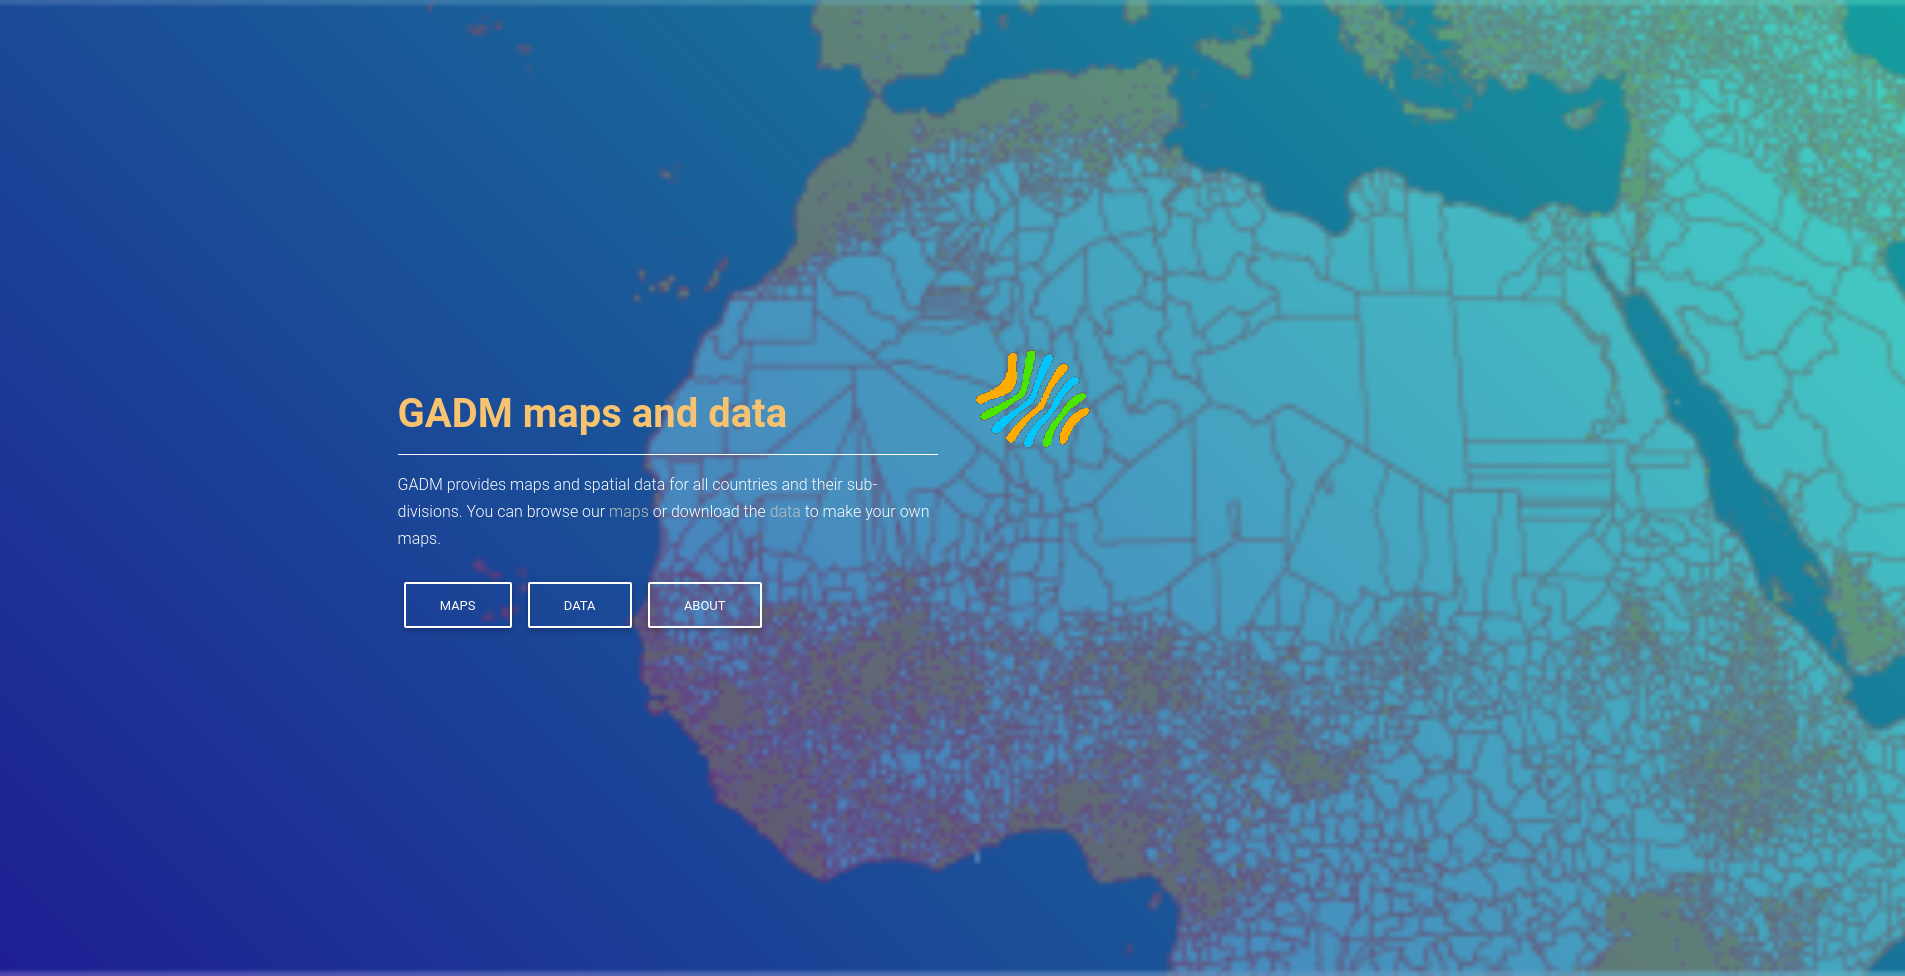
\includegraphics[width=\textwidth]{figures/gadm}
  \blfootnote{\url{https://gadm.org/}}
\end{frame}

\section[Aplicaciones Geoespaciales]{Aplicaciones Geoespaciales en la Era del Big Spatial Data}

\begin{frame}{Aplicaciones Geoespaciales}
    OpenTrees
    \centering
    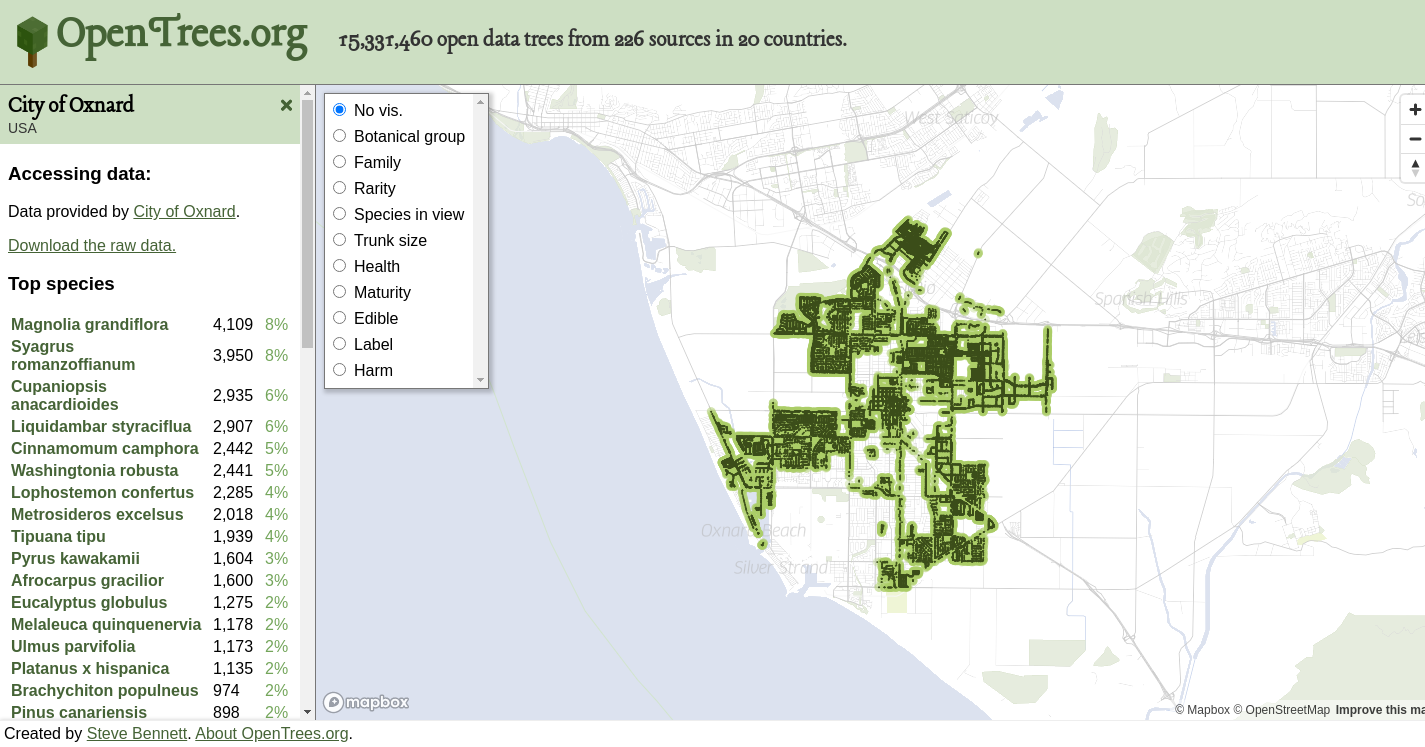
\includegraphics[width=\textwidth]{figures/opentree}
    \blfootnote{\url{http://opentrees.org/}}
\end{frame}

\begin{frame}{Aplicaciones Geoespaciales}
    CityGML
    \centering
    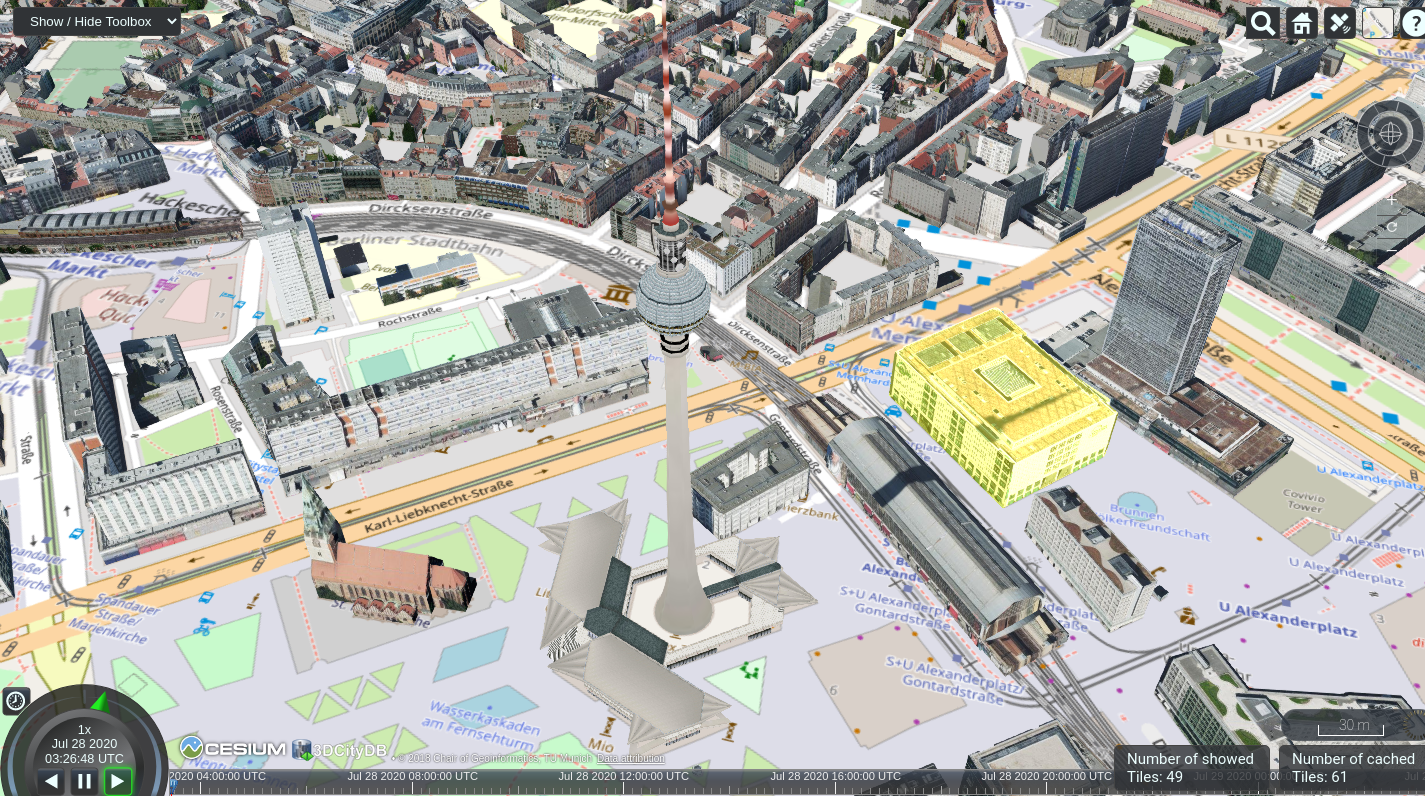
\includegraphics[width=0.95\textwidth]{figures/citygml}
    \blfootnote{\url{https://www.3dcitydb.org/}}
\end{frame}

\begin{frame}{Aplicaciones Geoespaciales}
    kepler.gl
    \centering
    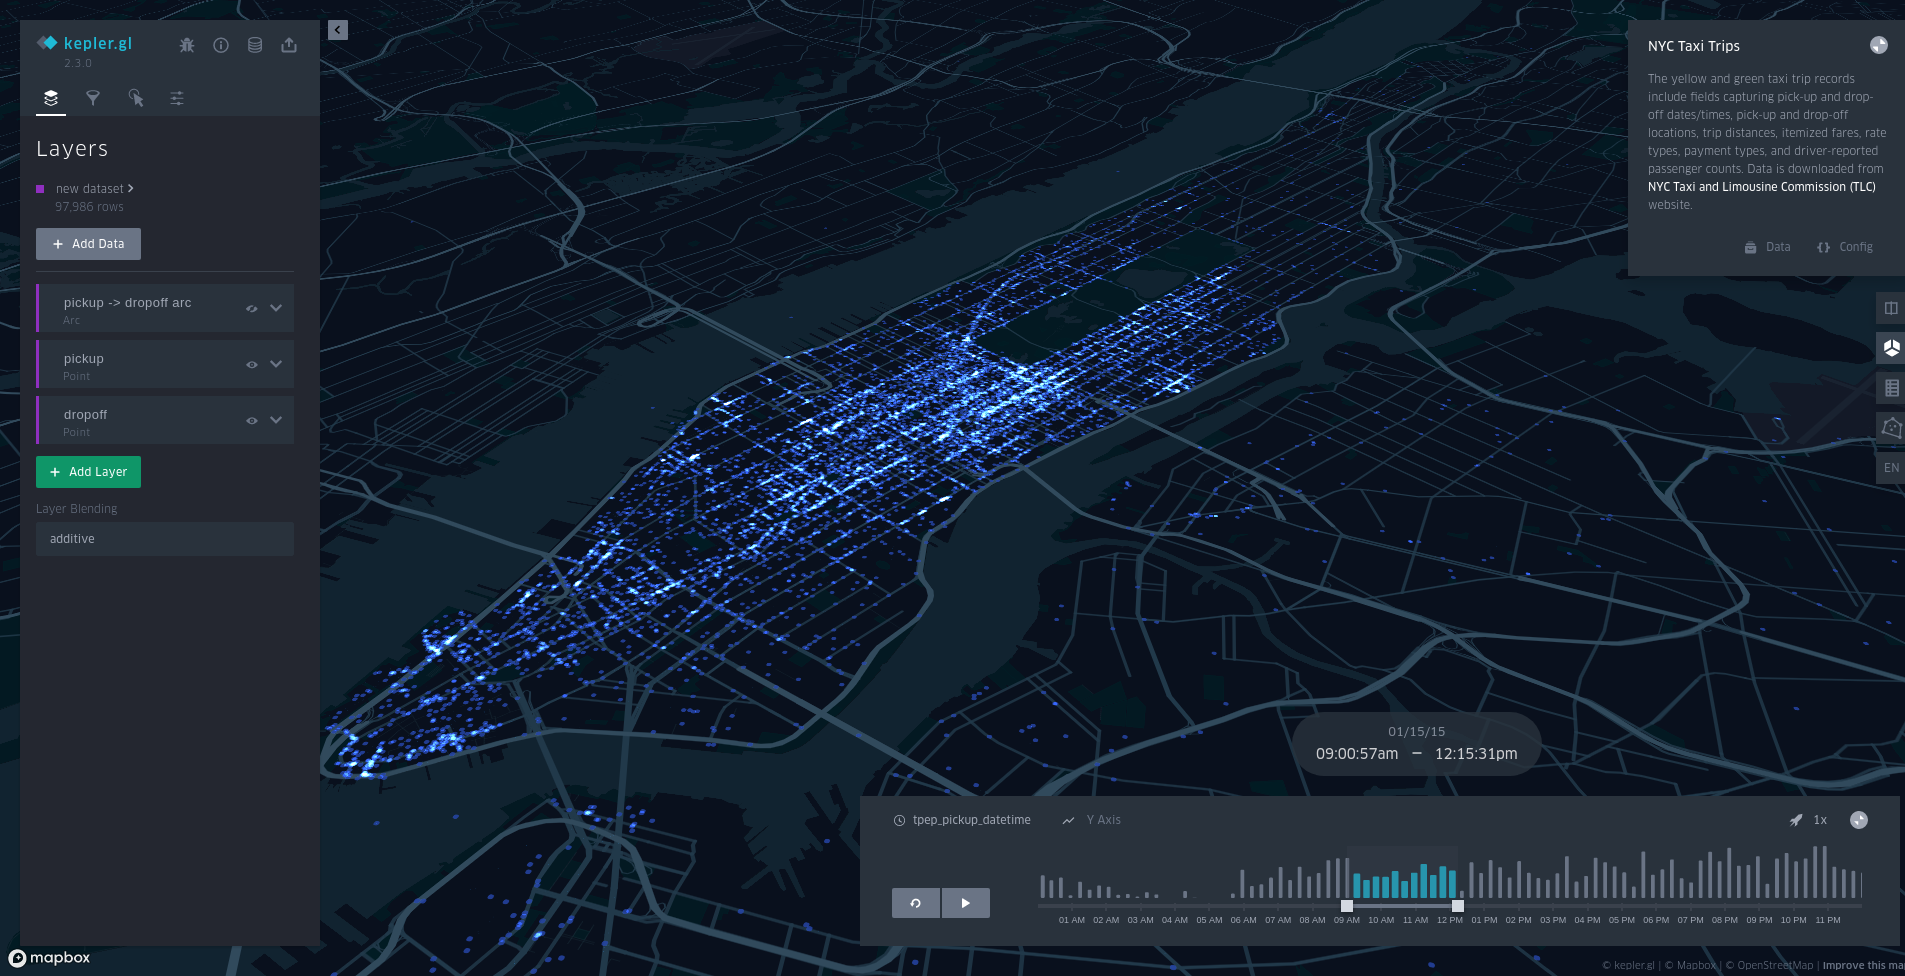
\includegraphics[width=\textwidth]{figures/kepler}
    \blfootnote{\url{https://kepler.gl/}}
\end{frame}

\begin{frame}{Aplicaciones Geoespaciales}
    London Santander Cycle Hire 
    \centering
    \includemedia[
        width=0.8\linewidth,
        height=0.5\linewidth,
        activate=pageopen,
        addresource=figures/london.mp4,
        flashvars={source=figures/london.mp4&autoPlay=true&loop=true}
    ]{}{VPlayer.swf}\\
    \blfootnote{https://twitter.com/CraigTaylorViz/status/874181612212297728?s=20}
\end{frame}

\begin{frame}{Aplicaciones Geoespaciales}
    Human Brain Project
    \centering
    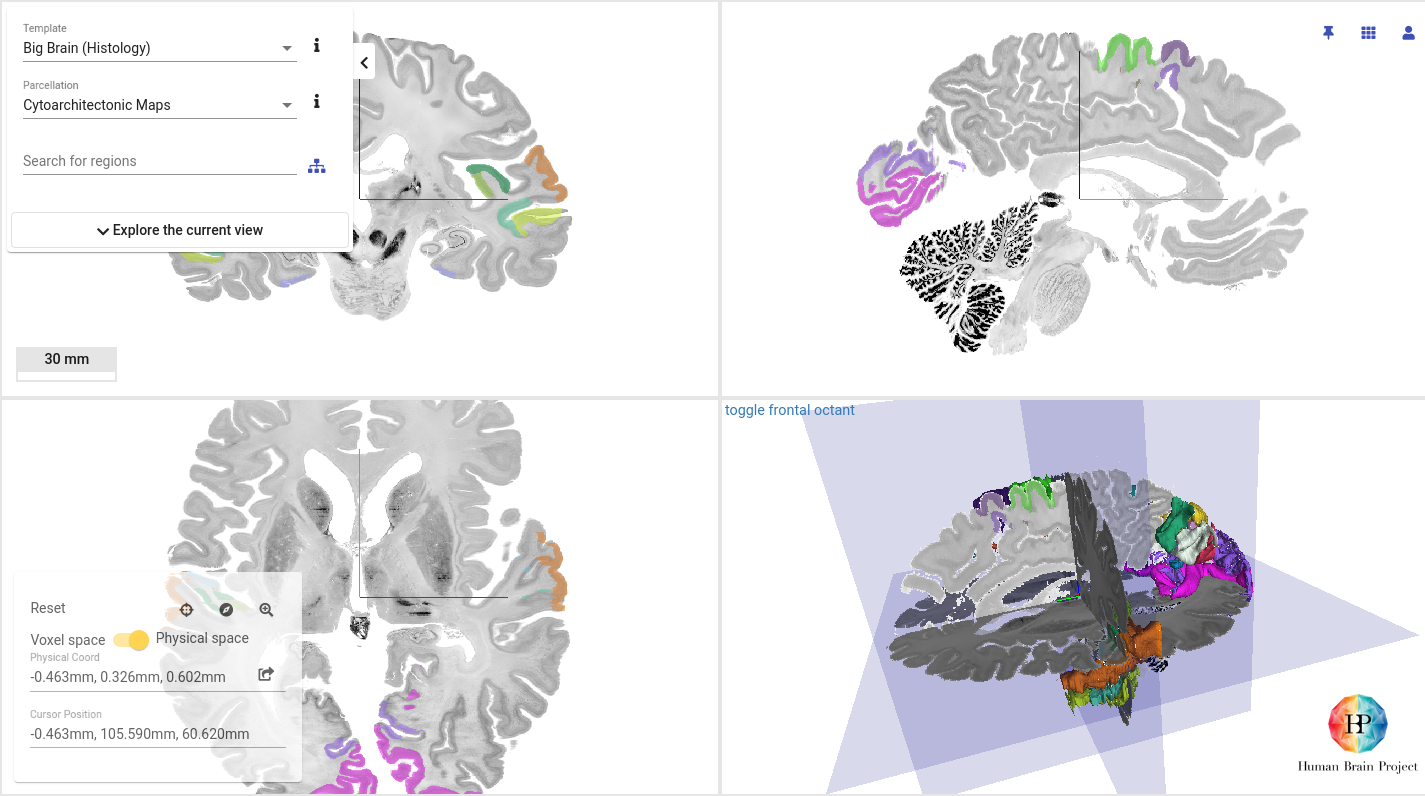
\includegraphics[width=0.95\textwidth]{figures/brain}
    \blfootnote{\url{https://interactive-viewer.apps.hbp.eu/}}
\end{frame}

\begin{frame}{Aplicaciones Geoespaciales}
    PlayerUnknown Battleground \hspace{2cm}
    \centering
    \includemedia[
        width=0.55\linewidth,
        height=0.55\linewidth,
        activate=pageopen,
        addresource=figures/games.mp4,
        flashvars={source=figures/games.mp4&autoPlay=true&loop=true}
    ]{}{VPlayer.swf}{\tiny \href{https://twitter.com/CraigTaylorViz/status/1270267416292048896?s=20}{@CraigTaylorViz}}\\
    \blfootnote{\url{https://www.kaggle.com/skihikingkevin/pubg-match-deaths}}
\end{frame}

\begin{frame}{Aplicaciones Geoespaciales}
    Zillow’s Home Value Prediction (Zestimate) 
    \centering
    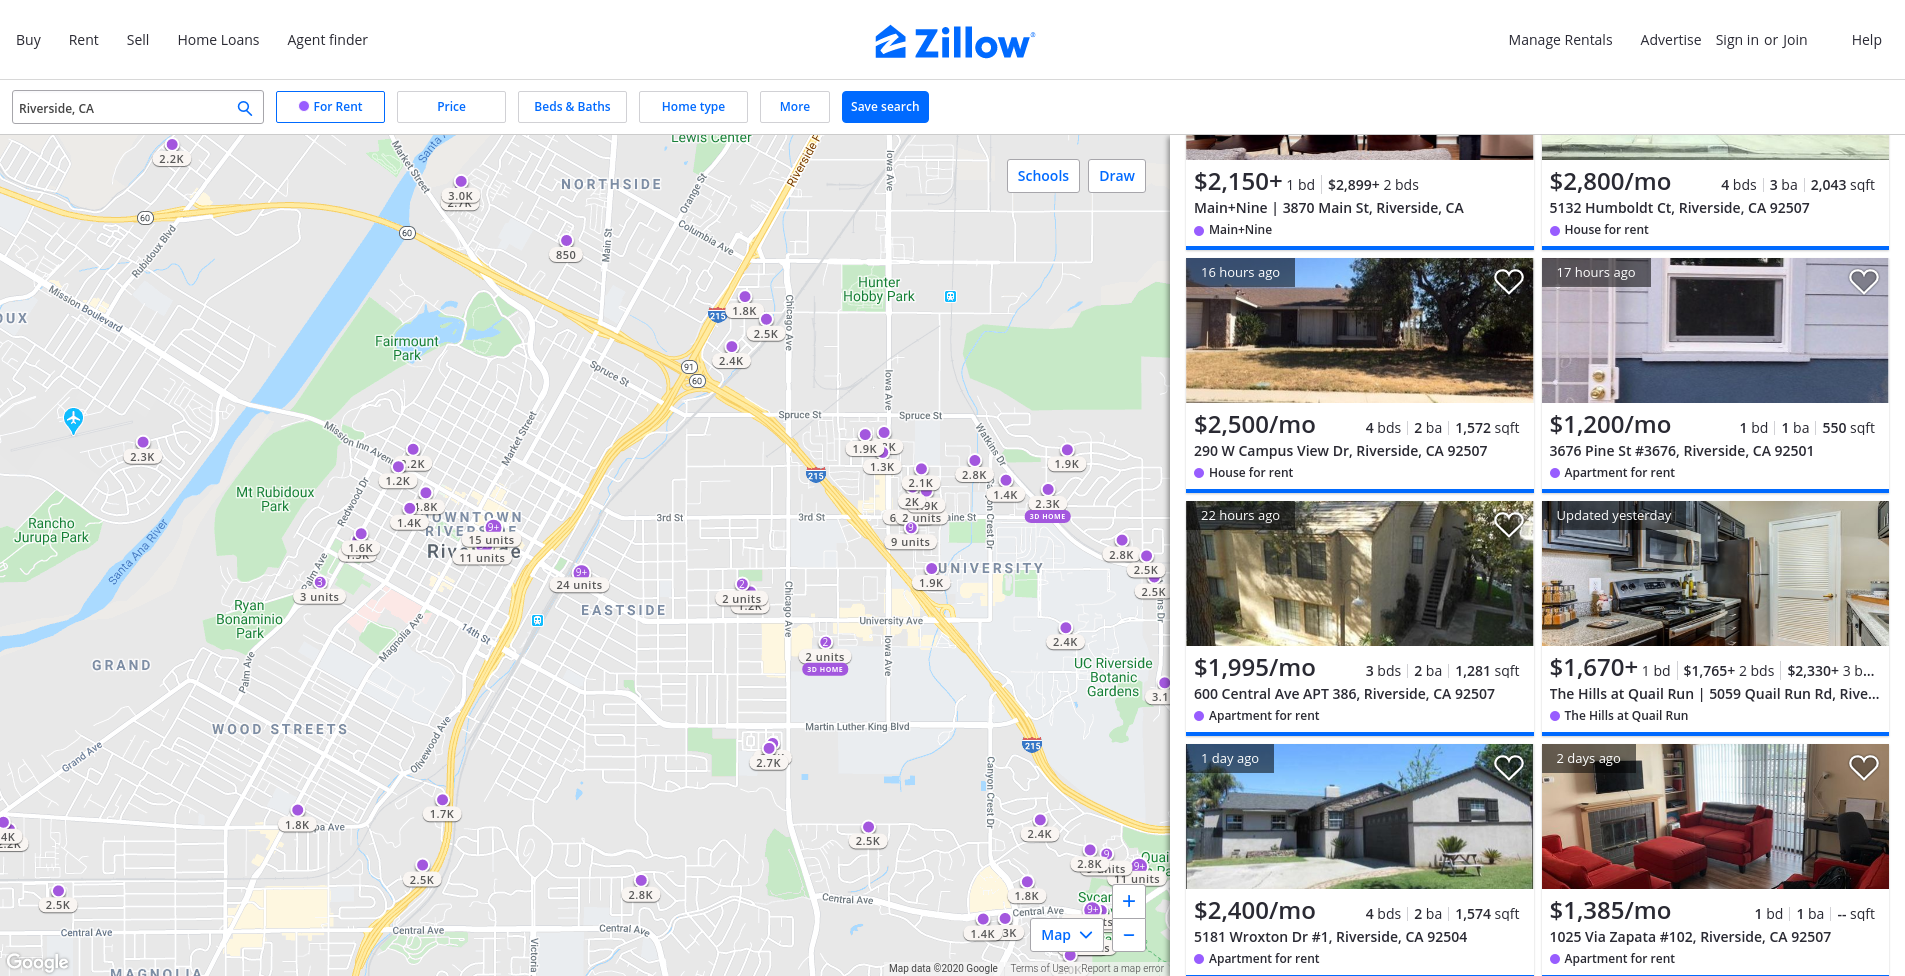
\includegraphics[width=\textwidth]{figures/zillow}\\
    \blfootnote{\url{https://www.kaggle.com/c/zillow-prize-1/}}
\end{frame}

\begin{frame}{Aplicaciones Geoespaciales}
    LandCoverNet
    \centering
    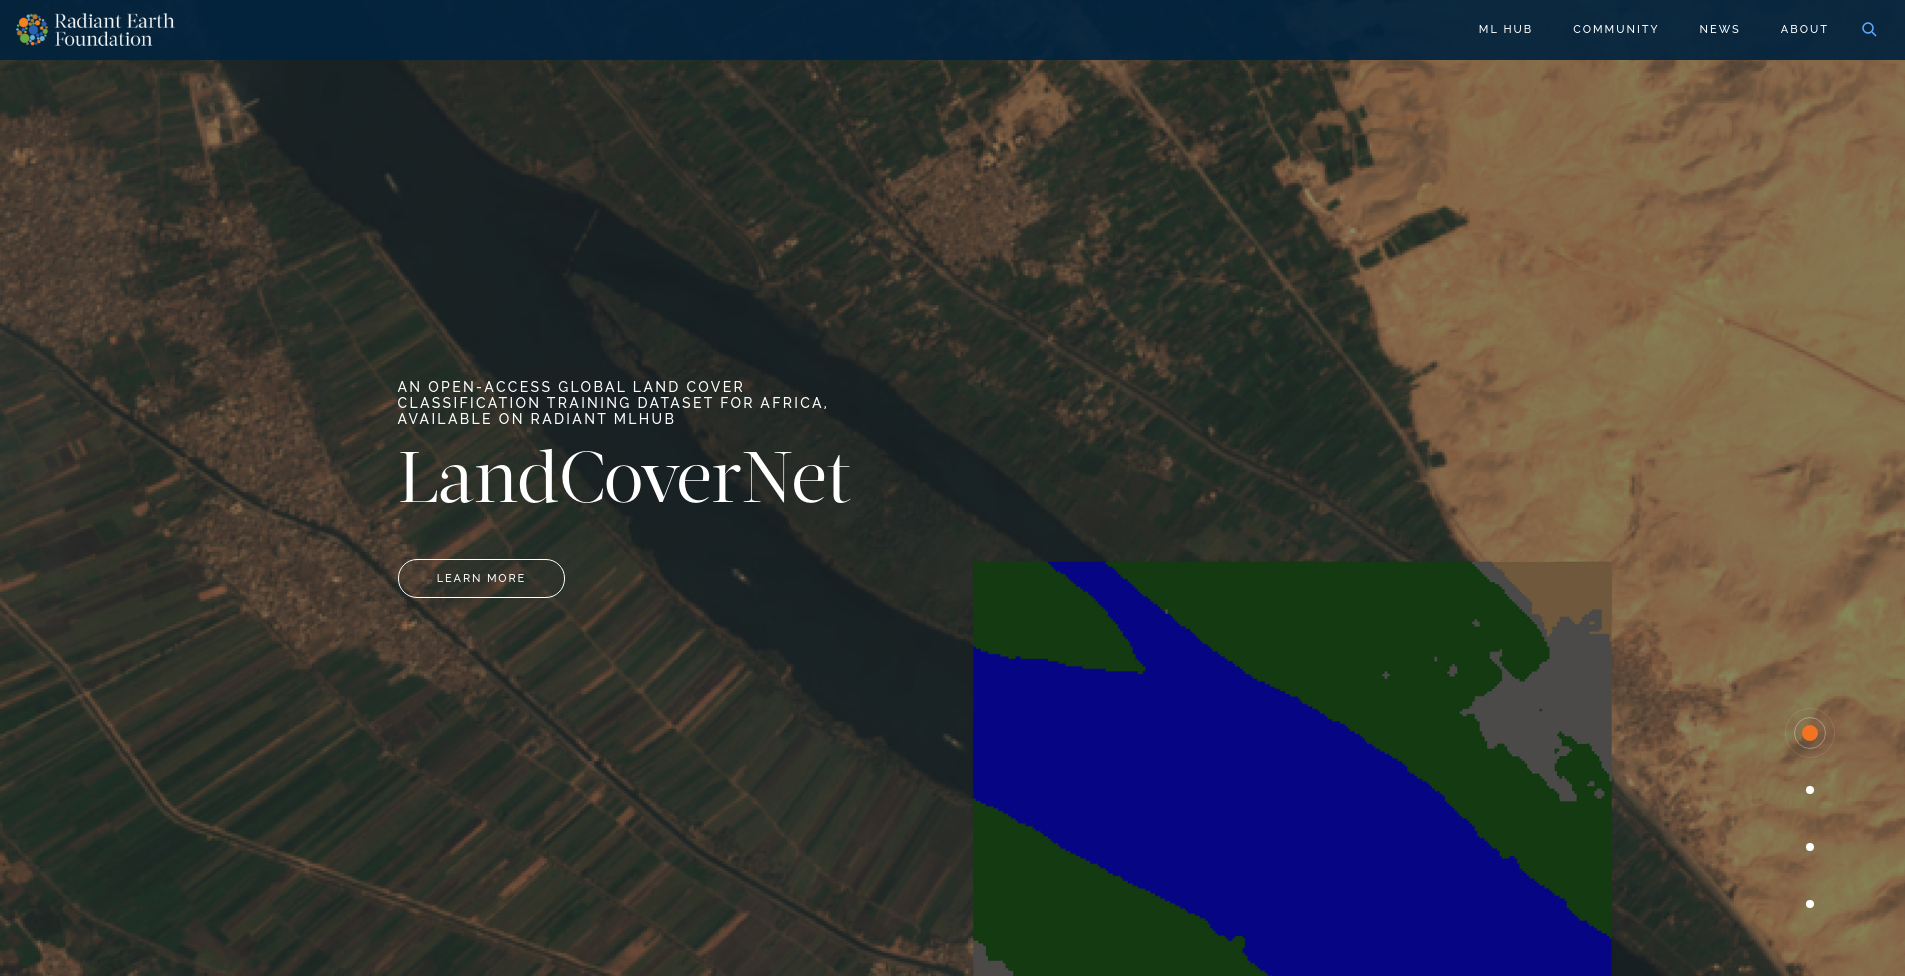
\includegraphics[width=0.95\textwidth]{figures/landcover}
    \blfootnote{\url{https://www.radiant.earth/}}
\end{frame}

\begin{frame}{Aplicaciones Geoespaciales}
    Agricultura de precision
    \centering
    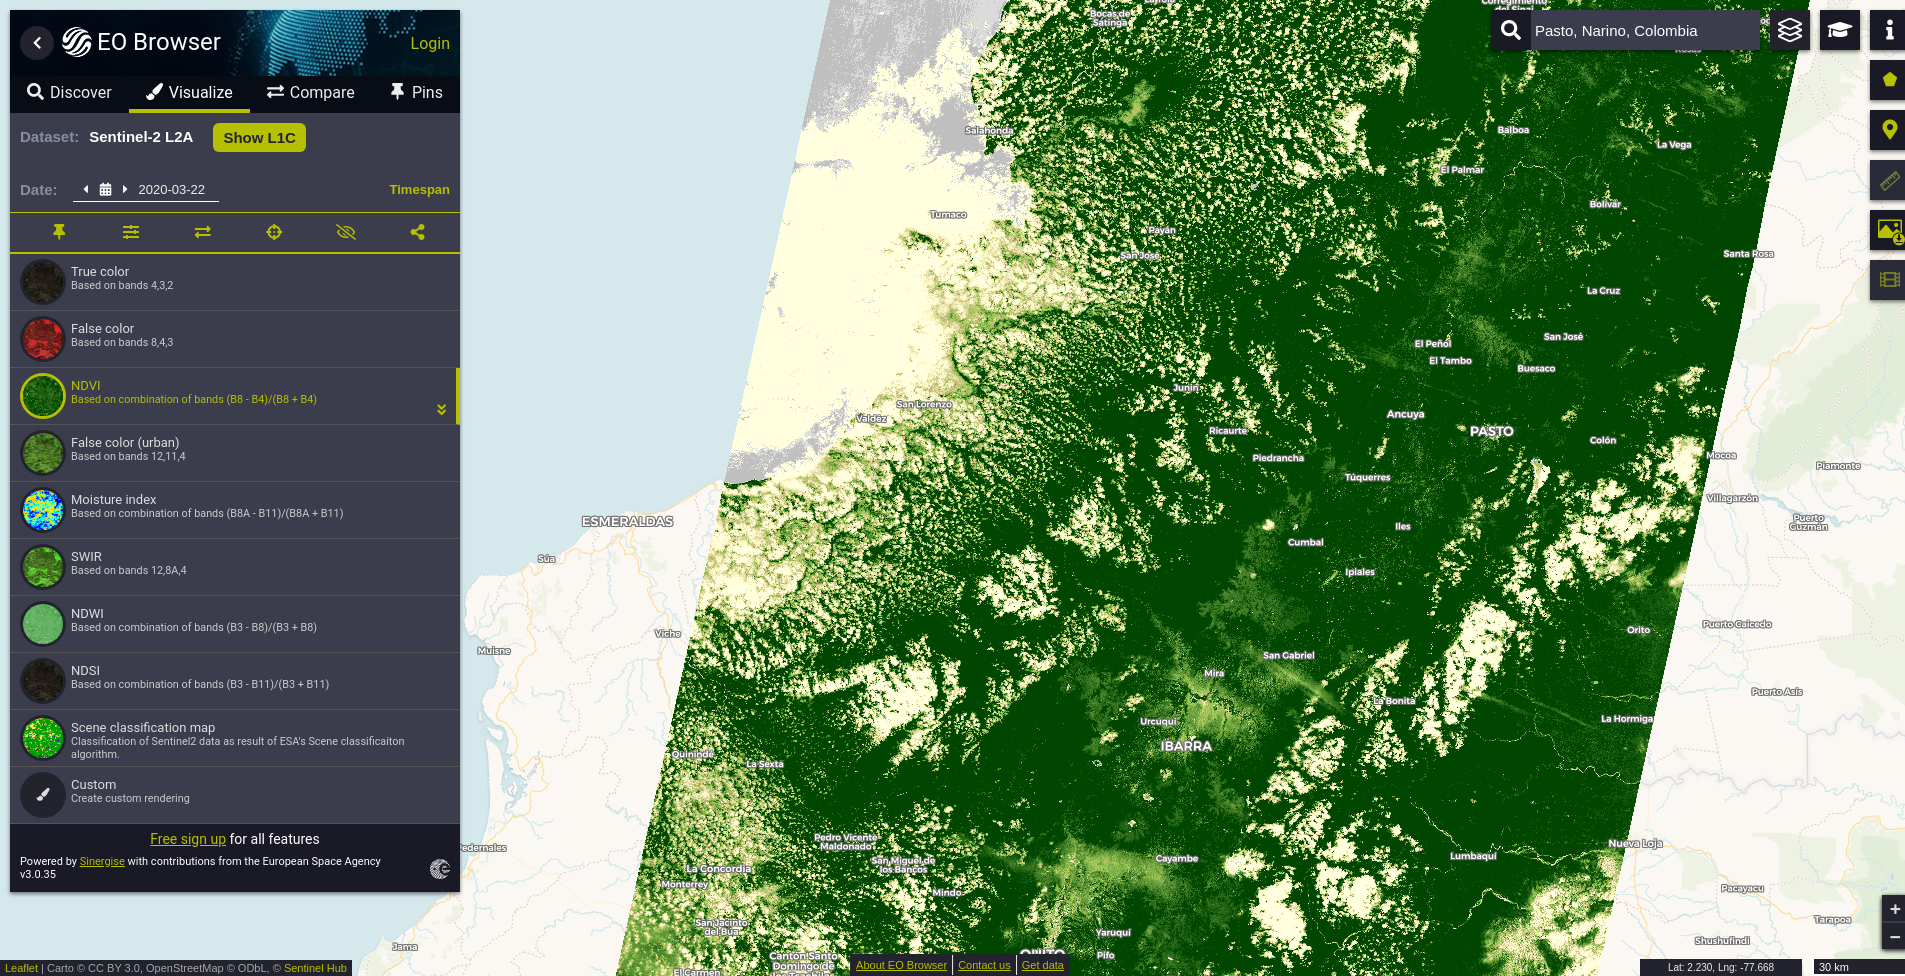
\includegraphics[width=0.95\textwidth]{figures/sentinelhub}\\
    \blfootnote{\url{https://apps.sentinel-hub.com/eo-browser/?zoom=7&lat=2.01009&lng=-78.85986&themeId=DEFAULT-THEME}}
\end{frame}

\begin{frame}{Aplicaciones Geoespaciales}
    Movebank \hspace{5cm}
    \centering
    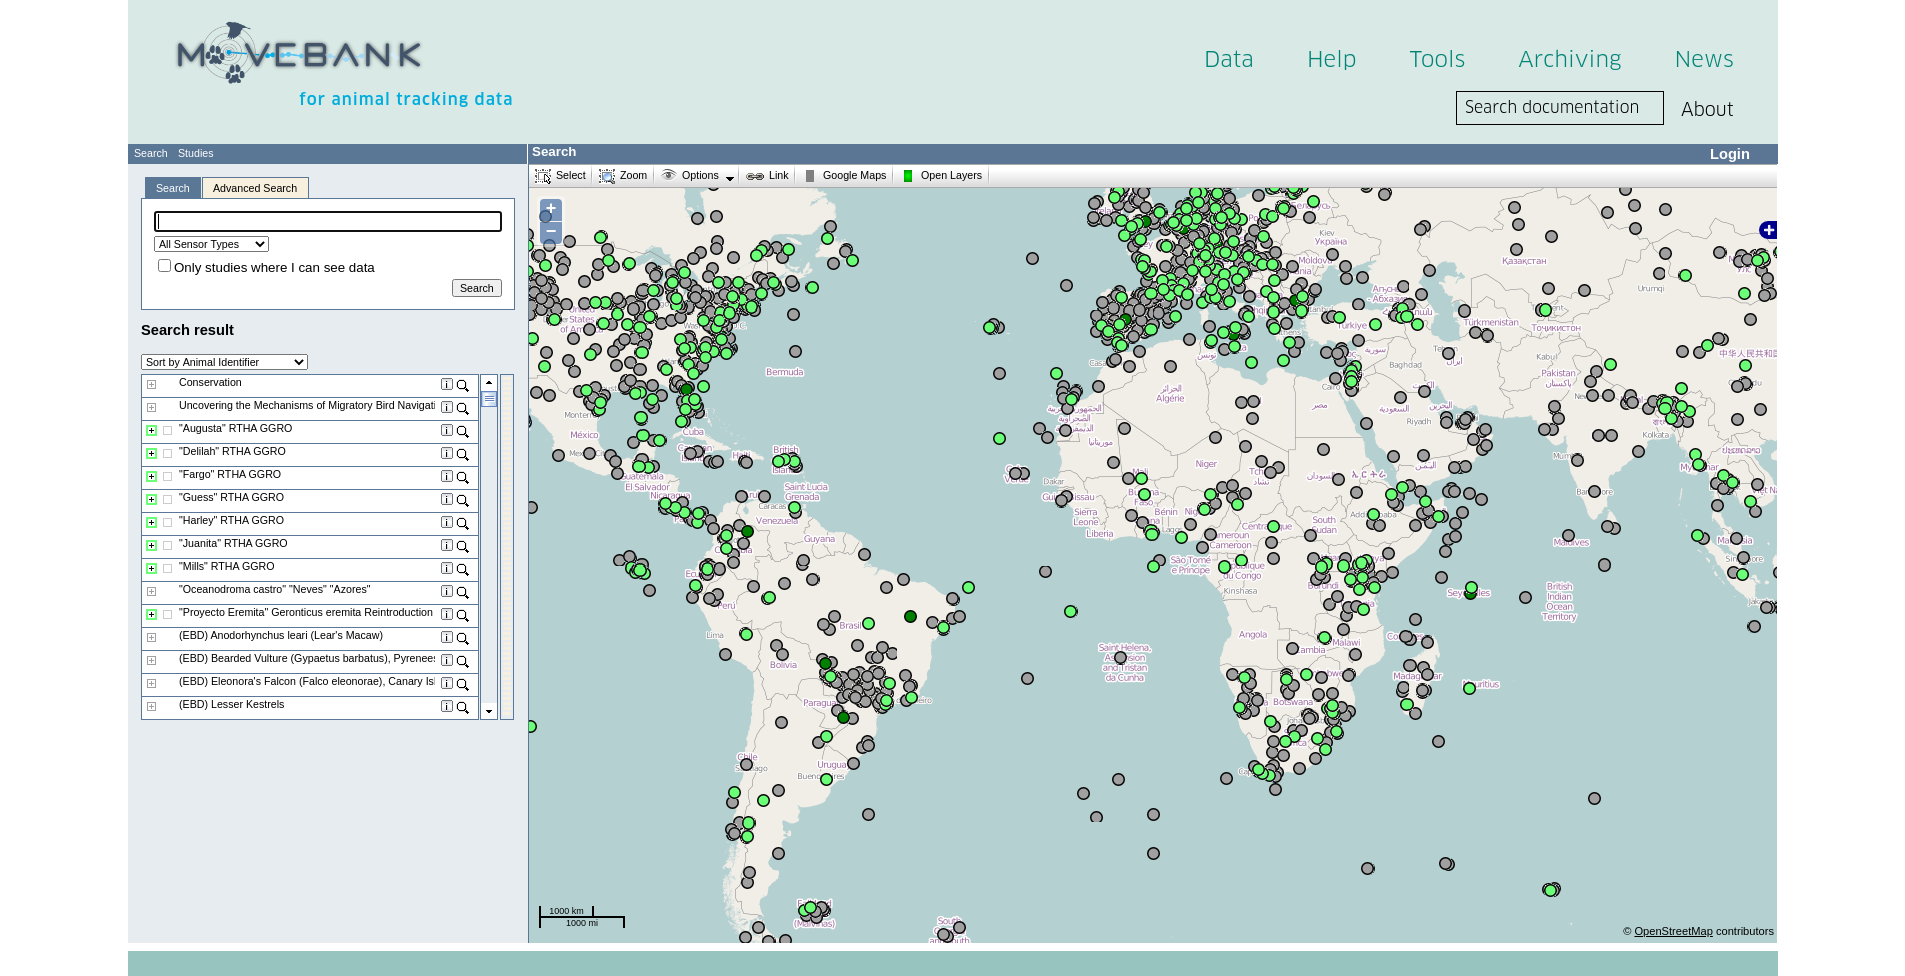
\includegraphics[width=\textwidth]{figures/movebank}\\
    \blfootnote{\url{https://www.movebank.org/}}
\end{frame}

\begin{frame}{Aplicaciones Geoespaciales}
    New York City Taxi Dataset  
    \centering
    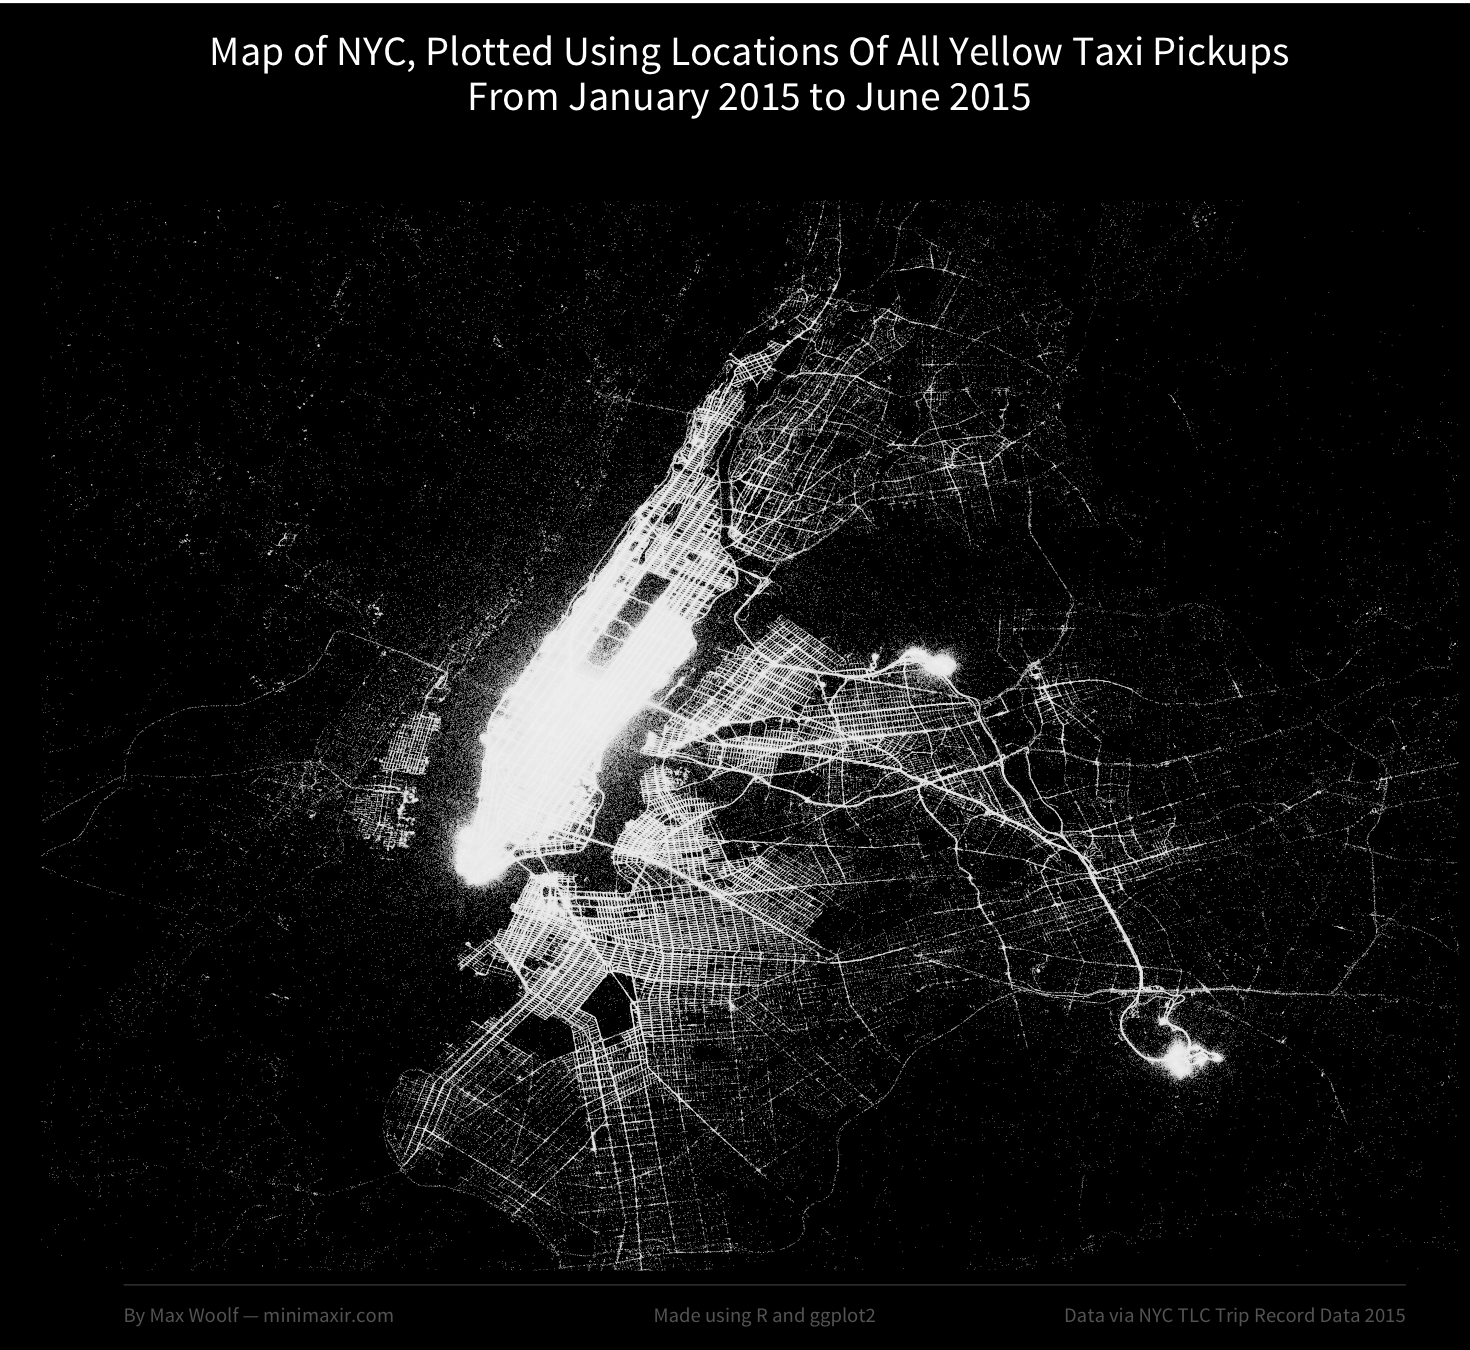
\includegraphics[width=0.6\textwidth]{figures/nytaxi}\\
    \blfootnote{\url{https://toddwschneider.com/posts/analyzing-1-1-billion-nyc-taxi-and-uber-trips-with-a-vengeance/}}
\end{frame}

\begin{frame}{Aplicaciones Geoespaciales}
    GeoSpark Sim
    \centering
    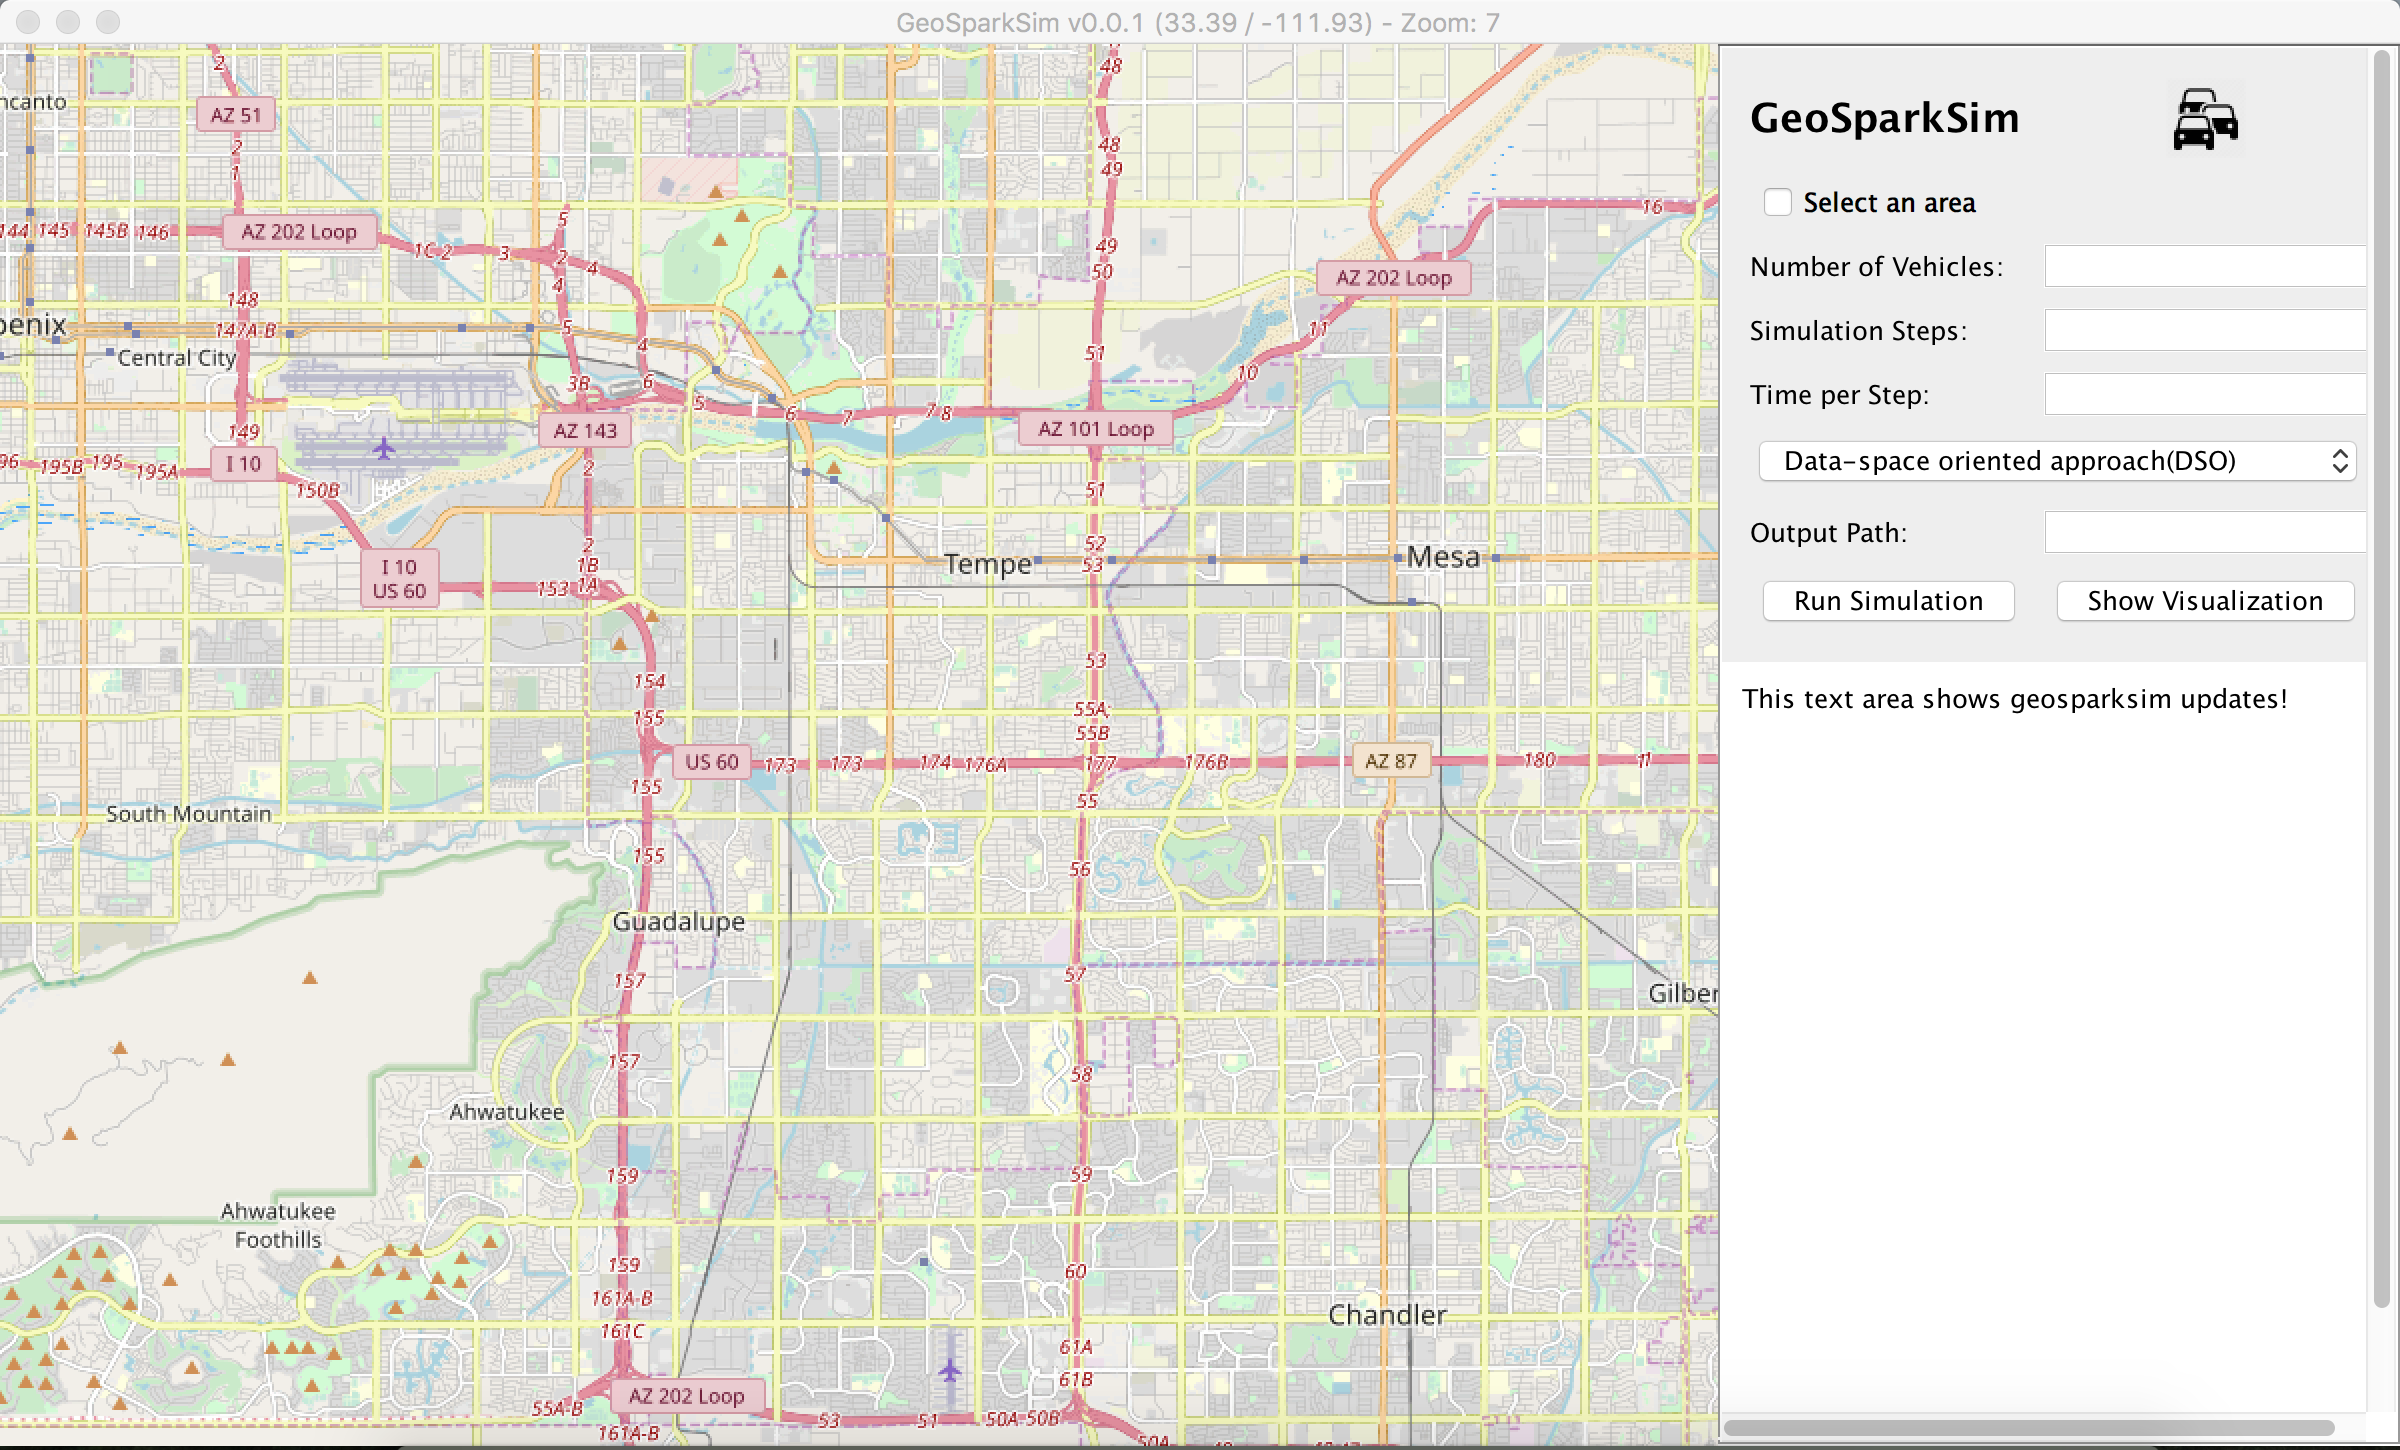
\includegraphics[width=0.95\textwidth]{figures/geosparksim}
    \blfootnote{\url{https://github.com/zishanfu/GeoSparkSim}}
\end{frame}

\begin{frame}{Aplicaciones Geoespaciales}
    Sidewalk Widths Toronto
    \centering
    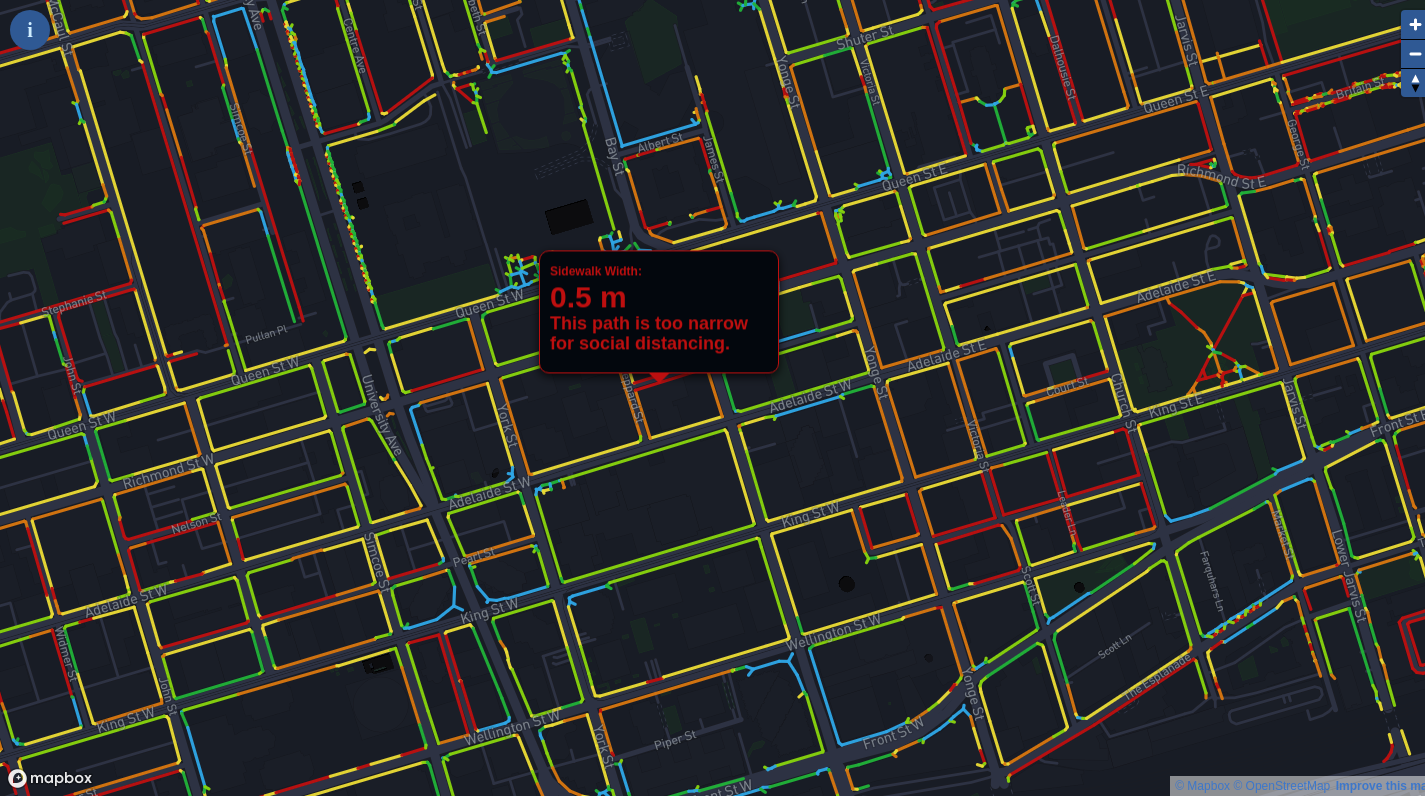
\includegraphics[width=0.95\textwidth]{figures/distancing}\\
    \blfootnote{\url{https://sharedstreets.github.io/sidewalkwidths-toronto}}
\end{frame}

\begin{frame}{Aplicaciones Geoespaciales}
    TectonixGEO Covid-19 tracking
    \centering
    \includemedia[
        width=0.8\linewidth,
        height=0.5\linewidth,
        activate=pageopen,
        addresource=figures/mobile2.mp4,
        flashvars={source=figures/mobile2.mp4}
    ]{}{VPlayer.swf}\\
    \blfootnote{\url{https://twitter.com/TectonixGEO/status/1242628347034767361?s=20}}
\end{frame}

\begin{frame}{Aplicaciones Geoespaciales}
    Truck Detection with Sentinel-2 during COVID-19 crisis
    \centering
    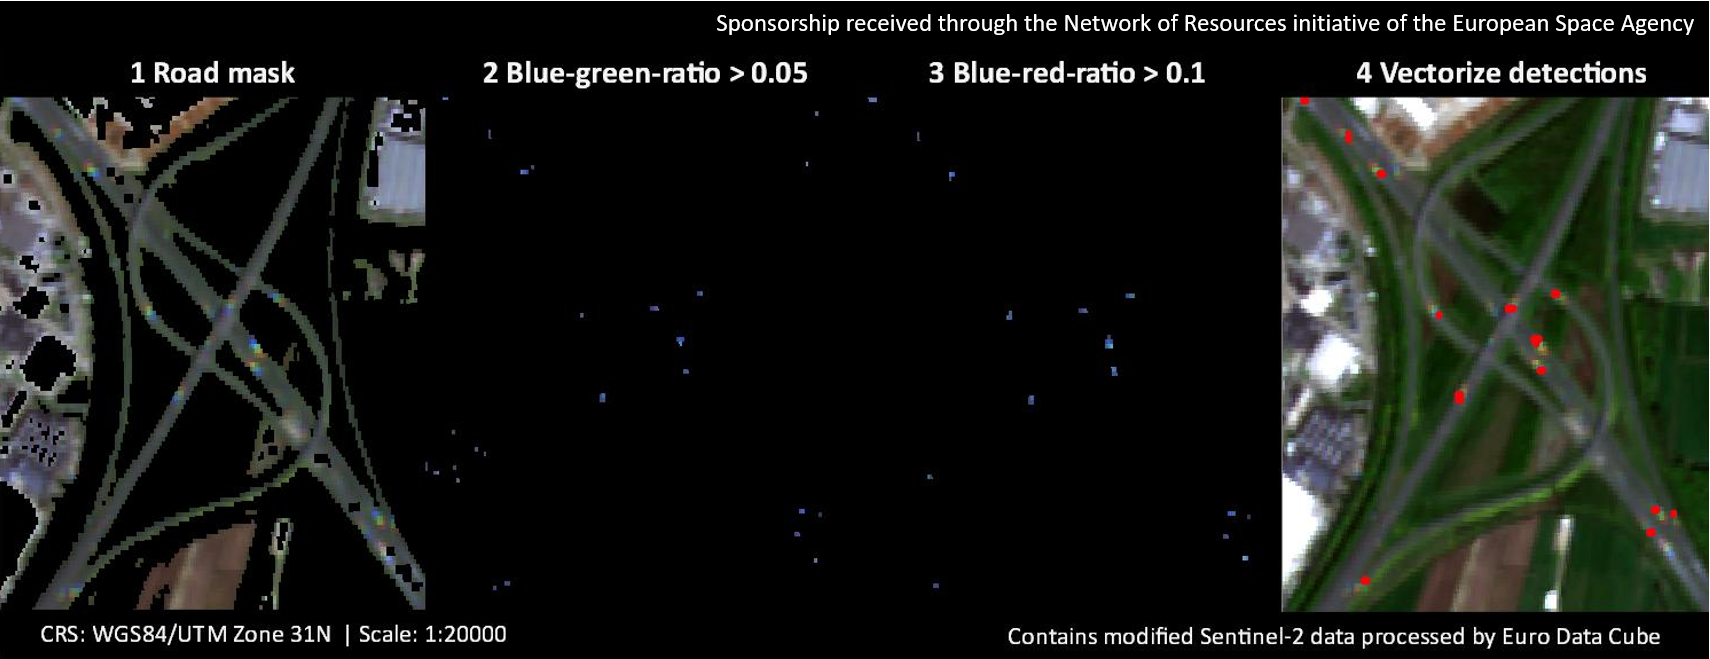
\includegraphics[width=0.95\textwidth]{figures/trucks}\\
    \blfootnote{\url{https://github.com/hfisser/Truck_Detection_Sentinel2_COVID19}}
\end{frame}

\section[Oportunidades y Desafios]{Aplicaciones Geoespaciales en la Era del Big Spatial Data: Oportunidades y Desafios}

\begin{frame}{Oportunidades y Desafios}
    Open Data Cube \\
    \centering
    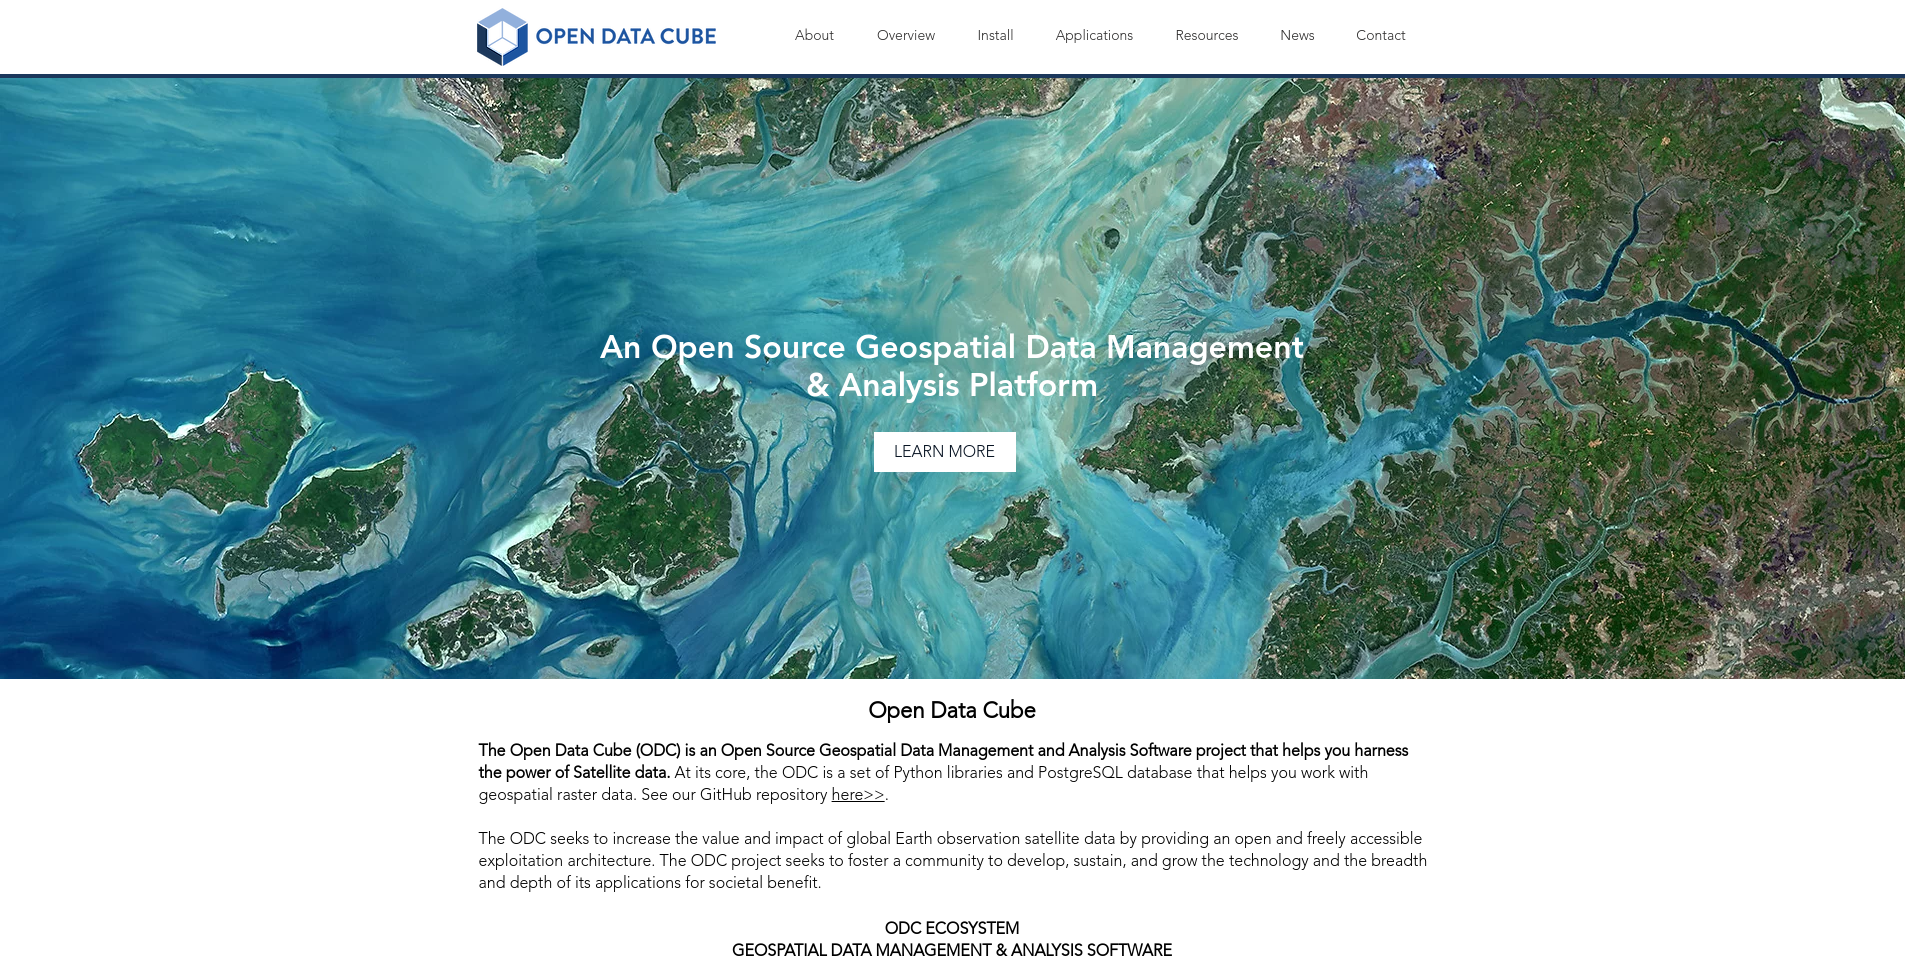
\includegraphics[width=0.95\textwidth]{figures/odc}\\
    \blfootnote{\url{https://www.opendatacube.org/}}
\end{frame}
\begin{frame}{Oportunidades y Desafios}
    Open Data Cube \\
    \centering
    \includemedia[
        width=0.66\linewidth,
        height=0.33\linewidth,
        activate=pageopen,
        addresource=figures/cube.mp4,
        flashvars={source=figures/cube.mp4&autoPlay=true&loop=true}
    ]{}{VPlayer.swf}
\end{frame}
\begin{frame}{Oportunidades y Desafios}
    Open Data Cube \\
    \centering
    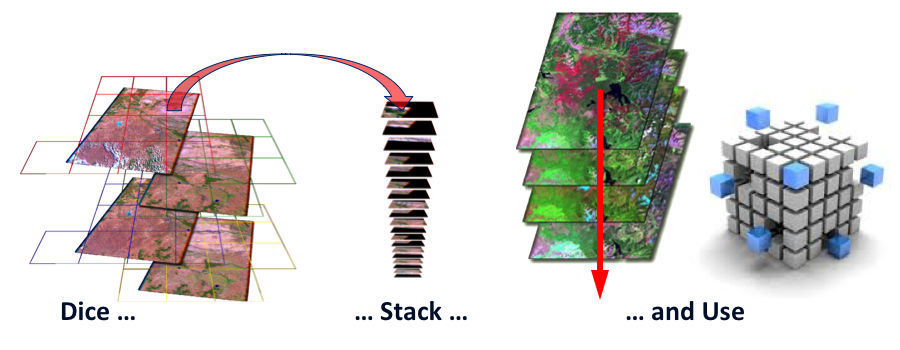
\includegraphics[width=0.95\textwidth]{figures/cube2}\\
\end{frame}

\begin{frame}{Oportunidades y Desafios}
    Mapillary \\
    \centering
    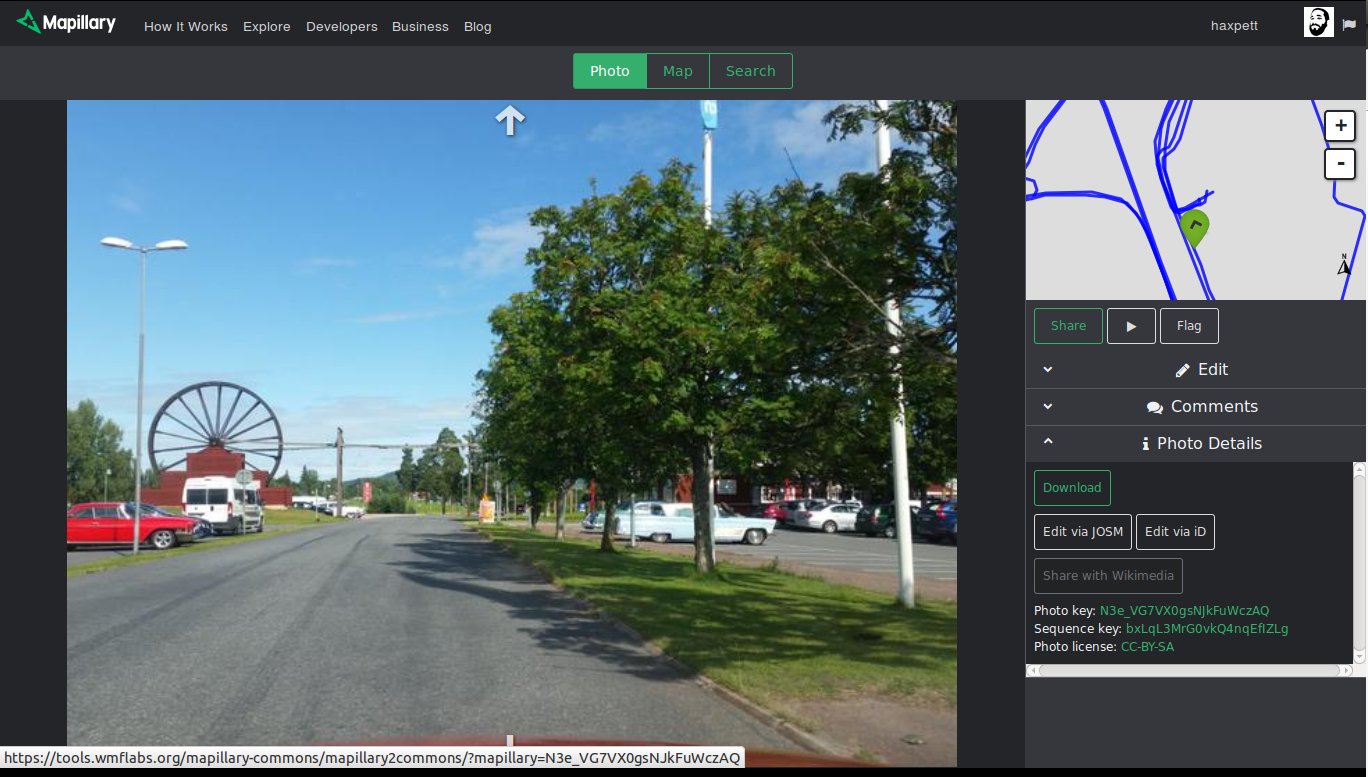
\includegraphics[width=0.95\textwidth]{figures/mapillary}\\
    \blfootnote{\url{https://www.mapillary.com/}}
\end{frame}
\begin{frame}{Oportunidades y Desafios}
    Computer vision \\
    \centering
    \includemedia[
        width=0.66\linewidth,
        height=0.33\linewidth,
        activate=pageopen,
        addresource=figures/vision.mp4,
        flashvars={source=figures/vision.mp4&autoPlay=true&loop=true}
    ]{}{VPlayer.swf}
\end{frame}
\begin{frame}{Oportunidades y Desafios}
    Mapillary Vistas Dataset \\
    \centering
    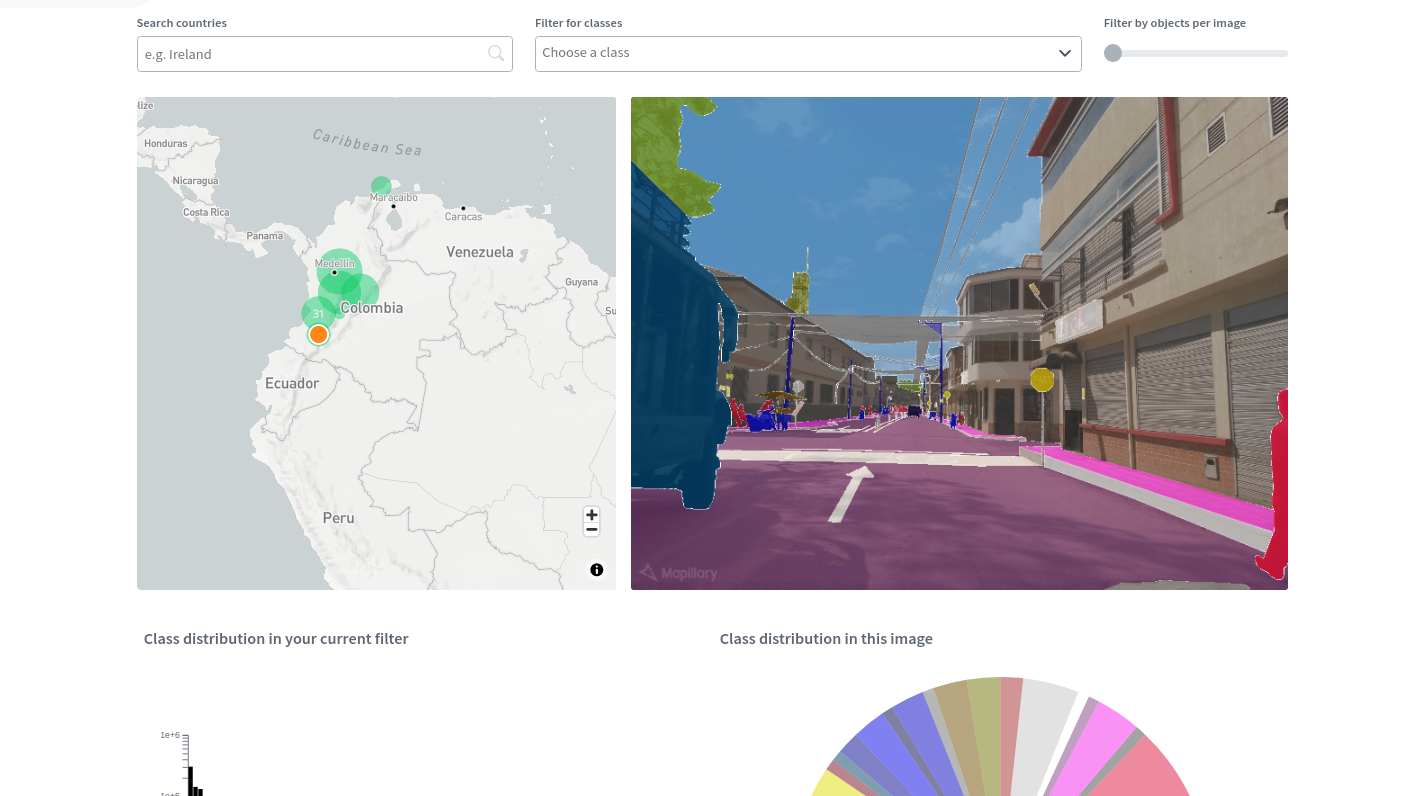
\includegraphics[width=0.95\textwidth]{figures/vistas}\\
    \blfootnote{\url{https://www.mapillary.com/dataset/vistas}}
\end{frame}

\begin{frame}{Oportunidades y Desafios}
    Super Resolution Imagery \\
    \centering
    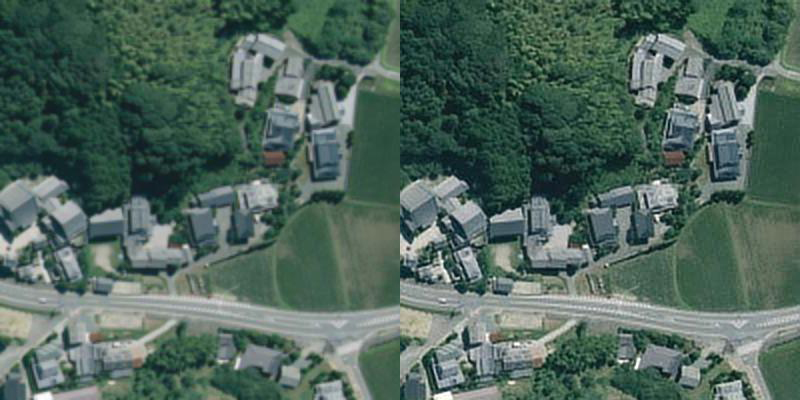
\includegraphics[width=0.5\textwidth]{figures/sr1}\\
    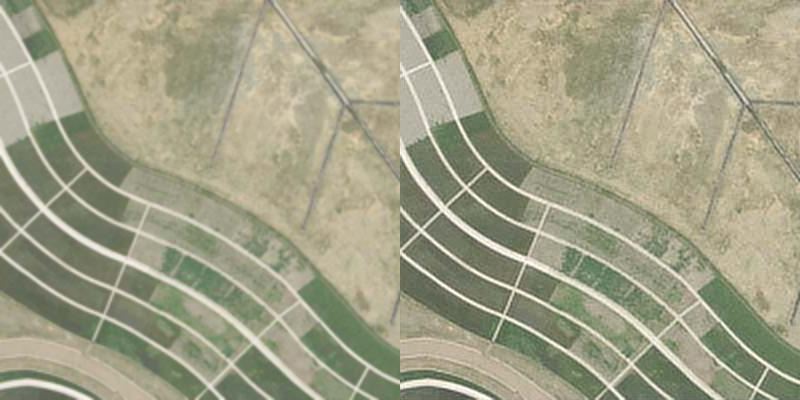
\includegraphics[width=0.5\textwidth]{figures/sr2}\\
    \blfootnote{\url{https://github.com/WarrenGreen/srcnn}}
\end{frame}
\begin{frame}{Oportunidades y Desafios}
    Super Resolution Imagery \\
    \centering
    \includemedia[
        width=0.5\linewidth,
        height=0.5\linewidth,
        activate=pageopen,
        addresource=figures/dem.mp4,
        flashvars={source=figures/dem.mp4&autoPlay=true&loop=true}
    ]{}{VPlayer.swf}
\end{frame}
\begin{frame}{Oportunidades y Desafios}
    EuroSat Dataset \\
    \centering
    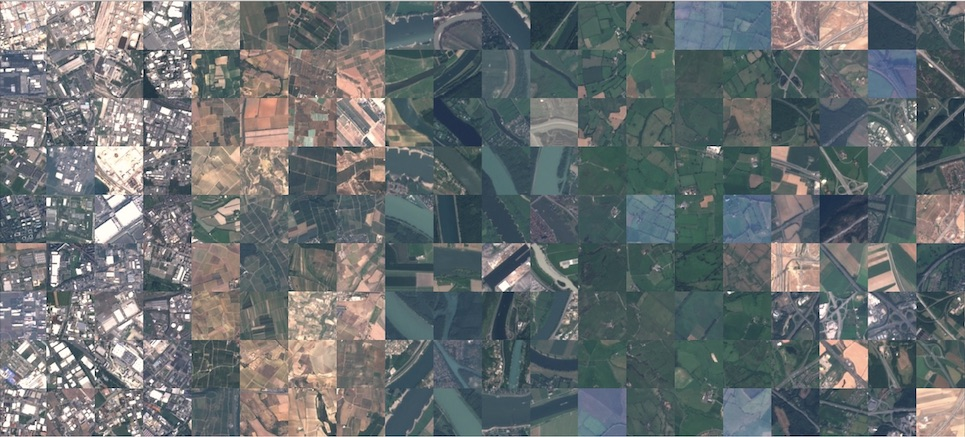
\includegraphics[width=0.95\textwidth]{figures/eurosat}\\
    \blfootnote{\url{http://madm.dfki.de/downloads}}
\end{frame}

\begin{frame}{Oportunidades y Desafios}
    OpenDroneMap \\
    \centering
    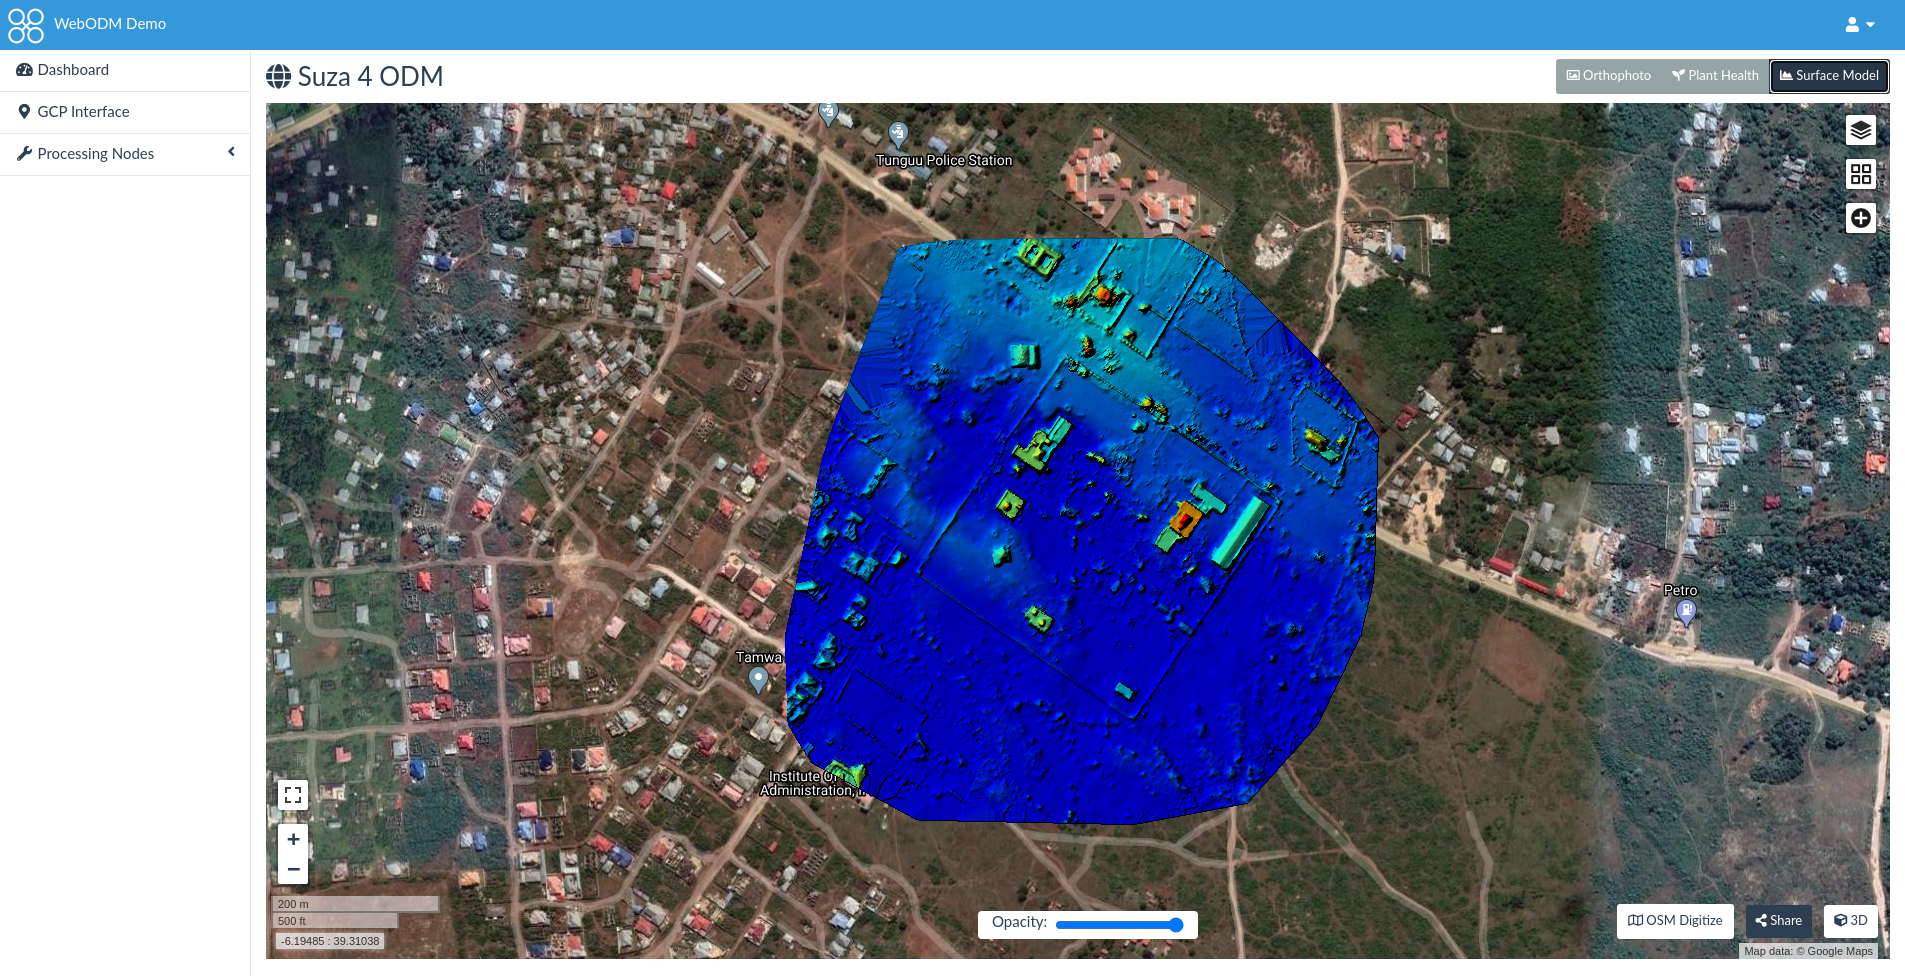
\includegraphics[width=0.95\textwidth]{figures/odm1}\\
    \blfootnote{\url{https://www.opendronemap.org/}}
\end{frame}
\begin{frame}{Oportunidades y Desafios}
    ArduPilot \\
    \centering
    \includemedia[
        width=0.5\linewidth,
        height=0.5\linewidth,
        activate=pageopen,
        addresource=figures/ardupilot.mp4,
        flashvars={source=figures/ardupilot.mp4&autoPlay=true&loop=true}
    ]{}{VPlayer.swf}
\end{frame}
\begin{frame}{Oportunidades y Desafios}
    HIS de bajo costo \\
    \centering
    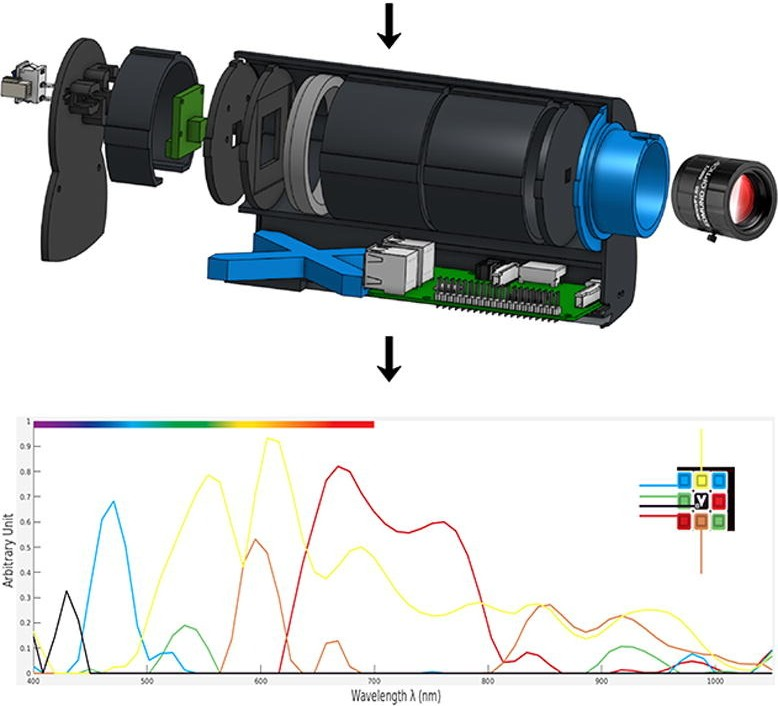
\includegraphics[width=0.6\textwidth]{figures/spectometer}\\
    \blfootnote{\url{https://www.sciencedirect.com/science/article/pii/S2468067219300513}}
\end{frame}

\begin{frame}{Preguntas???}
    \centering
    \includegraphics[trim=0cm 17.5cm 0cm 12.5cm, clip,width=0.5\textwidth]{figures/sol}
\end{frame}

\end{document}

